                                                                                                                                                                                  %%%%%%%%%%%%%%%%%%%%%%%%%%%%%%%%%%%%%%%%%
% Masters/Doctoral Thesis 
% LaTeX Template
% Version 2.2 (21/11/15)
%
% This template has been downloaded from:
% http://www.LaTeXTemplates.com
%
% Version 2.x major modifications by:
% Vel (vel@latextemplates.com)
%
% This template is based on a template by:
% Steve Gunn (http://users.ecs.soton.ac.uk/srg/softwaretools/document/templates/)
% Sunil Patel (http://www.sunilpatel.co.uk/thesis-template/)
%
% Template license:
% CC BY-NC-SA 3.0 (http://creativecommons.org/licenses/by-nc-sa/3.0/)
%
%%%%%%%%%%%%%%%%%%%%%%%%%%%%%%%%%%%%%%%%%

%----------------------------------------------------------------------------------------
%	PACKAGES AND OTHER DOCUMENT CONFIGURATIONS
%----------------------------------------------------------------------------------------

\documentclass[
11pt, % The default document fmont size, options: 10pt, 11pt, 12pt
oneside, % Two side (alternating margins) for binding by default, uncomment to switch to one side
spanish, % ngerman for German
singlespacing, % Single line spacing, alternatives: onehalfspacing or doublespacing
%draft, % Uncomment to enable draft mode (no pictures, no links, overfull hboxes indicated)
%nolistspacing, % If the document is onehalfspacing or doublespacing, uncomment this to set spacing in lists to single
%liststotoc, % Uncomment to add the list of figures/tables/etc to the table of contents
%toctotoc, % Uncomment to add the main table of contents to the table of contents
parskip, % Uncomment to add space between paragraphs
%nohyperref, % Uncomment to not load the hyperref package
headsepline, % Uncomment to get a line under the header
]{MastersDoctoralThesis} % The class file specifying the document structure


\usepackage[utf8]{inputenc} % Required for inputting international characters
\usepackage[T1]{fontenc} % Output font encoding for international characters
%\usepackage{parskip} % Space between paragraphs
\usepackage{palatino} % Use the Palatino font by default
\hyphenation{HTCondor} % evita que conrte la palara en salto de linea
% \hypersetup{allcolors=black} % evita colores de hypertexto pasa todo a negro
%\hypersetup{colorlinks=false}
\usepackage{titlesec}
\titleformat{\chapter}{}{}{0em}{\bf\LARGE}

\usepackage{listings} %code snipets

\usepackage[backend=bibtex,style=authoryear,natbib=true]{biblatex} % User the bibtex backend with the authoryear citation style (which resembles APA)

\addbibresource{referencias.bib} % The filename of the bibliography

\usepackage[autostyle=true]{csquotes} % Required to generate language-dependent quotes in the bibliography
\usepackage{placeins}
\usepackage{url}
\usepackage{hyperref}
%----------------------------------------------------------------------------------------
%	MARGIN SETTINGS
%----------------------------------------------------------------------------------------

\geometry{
	paper=a4paper, % Change to letterpaper for US letter
	inner=2.5cm, % Inner margin
	outer=3.8cm, % Outer margin
	bindingoffset=2cm, % Binding offset
	top=1.5cm, % Top margin
	bottom=1.5cm, % Bottom margin
	%showframe,% show how the type block is set on the page
}

%----------------------------------------------------------------------------------------
%	THESIS INFORMATION
%----------------------------------------------------------------------------------------

\thesistitle{Evaluación de uso de un cluster oportunista basados en sistemas operativos heterogéneos y HTCondor.} % Your thesis title, this is used in the title and abstract, print it elsewhere with \ttitle
\supervisor{Msc. Jairo \textsc{Serrano}} % Your supervisor's name, this is used in the title page, print it elsewhere with \supname
\examiner{} % Your examiner's name, this is not currently used anywhere in the template, print it elsewhere with \examname
\degree{Ingeniero de Sistemas} % Your degree name, this is used in the title page and abstract, print it elsewhere with \degreename
\author{Carlos \textsc{Buelvas Montes}} % Your name, this is used in the title page and abstract, print it elsewhere with \authorname
\addresses{} % Your address, this is not currently used anywhere in the template, print it elsewhere with \addressname

\subject{Computer Sciences} % Your subject area, this is not currently used anywhere in the template, print it elsewhere with \subjectname
\keywords{} % Keywords for your thesis, this is not currently used anywhere in the template, print it elsewhere with \keywordnames
\university{\href{http://www.unitecnologica.edu.co}{Universidad Tecnológica de Bolívar}} % Your university's name and URL, this is used in the title page and abstract, print it elsewhere with \univname
\department{\href{http://programas.unitecnologica.edu.co/ingenieria-de-sistemas}{Programa de Ingeniería de Sistemas}} % Your department's name and URL, this is used in the title page and abstract, print it elsewhere with \deptname
\group{\href{http://investigaciones.unitecnologica.edu.co/grupos/investigacion-tecnologias-aplicadas-sistemas-informacion}{GRITAS}} % Your research group's name and URL, this is used in the title page, print it elsewhere with \groupname
\faculty{\href{http://programas.unitecnologica.edu.co/facultad-de-ingenieria}{Facultad de Ingeniería}} % Your faculty's name and URL, this is used in the title page and abstract, print it elsewhere with \facname

\hypersetup{pdftitle=\ttitle} % Set the PDF's title to your title
\hypersetup{pdfauthor=\authorname} % Set the PDF's author to your name
\hypersetup{pdfkeywords=\keywordnames} % Set the PDF's keywords to your keywords
% inicio del documento
\begin{document}

\frontmatter % Use roman page numbering style (i, ii, iii, iv...) for the pre-content pages

\pagestyle{plain} % Default to the plain heading style until the thesis style is called for the body content

%----------------------------------------------------------------------------------------
%	TITLE PAGE
%----------------------------------------------------------------------------------------

\begin{titlepage}
\begin{center}

\textsc{\LARGE \univname}\\[1.5cm] % University name
\textsc{\Large Trabajo de Grado}\\[0.5cm] % Thesis type

\HRule \\[0.4cm] % Horizontal line
{\huge \bfseries \ttitle}\\[0.4cm] % Thesis title
\HRule \\[1.5cm] % Horizontal line
 
\begin{minipage}{0.4\textwidth}
\begin{flushleft} \large
\emph{Autor:}\\
\authorname
\end{flushleft}
\end{minipage}
\begin{minipage}{0.4\textwidth}
\begin{flushright} \large
\emph{Director:} \\
\supname
\end{flushright}
\end{minipage}\\[3cm]
 
\large \textit{Trabajo de grado entregado como requisito\\ para el titulo de  \degreename}\\[0.3cm] % University requirement text
\textit{Como parte del grupo de investigación}\\[0.4cm]
\groupname\\\facname\\[2cm] % Research group name and department name
 
{\large \today}\\[4cm] % Date
%\includegraphics{Logo} % University/department logo - uncomment to place it
 
\vfill
\end{center}
\end{titlepage}

%----------------------------------------------------------------------------------------
%	DECLARATION PAGE
%----------------------------------------------------------------------------------------

\begin{declaration}
\addchaptertocentry{}
\title{Declaración de autoría}

\noindent Yo, \authorname, declaro que este trabajo de grado, \enquote{\ttitle} y el trabajo realizado son de mi autoría. Confirmo que:

\begin{itemize} 
\item Este trabajo fue realizado parcial o total mente como estudiante de pregado de esta universidad.
\item Donde se consulta el trabajo publicado de otros, se hace la respectiva atribución.
\item Reconozco las principales fuentes de ayuda para este trabajo.
\item Este trabajo fue realizado bajo la supervisión del Msc Jairo Serrano, quien me guío y orientó en el proceso.\\
\end{itemize}
 
\noindent Firma:\\
\rule[0.5em]{25em}{0.5pt} % This prints a line for the signature
 
\noindent Fecha:\\
\rule[0.5em]{25em}{0.5pt} % This prints a line to write the date
\end{declaration}

\cleardoublepage

%----------------------------------------------------------------------------------------
%	QUOTATION PAGE
%----------------------------------------------------------------------------------------

\vspace*{0.2\textheight}

\noindent\enquote{\itshape Las grandes ideas, de grandes hombres en el mundo, que pueden llevar al progreso y la evolución del mismo, por lo general son impedidas por una sola cosa...

El resto de los hombres.}\bigbreak

\hfill Thomas Hamillton (Black Sails)

%----------------------------------------------------------------------------------------
%	ABSTRACT PAGE
%----------------------------------------------------------------------------------------

\begin{abstract}
\addchaptertocentry{\abstractname} % Add the abstract to the table of contents

In the technological university of Bolivar, there is a high demand on machines to handle a huge amount of data, in order to process that workload, It uses a grid system, a cluster to provide an infrastructure support to handle that work. To achieve this goal implements the use of HTCondor, a software to control the jobs assigned to this cluster, allowing to perform different tasks, follow the job process, define architecture, even a operative system for the job execution. \\
We test the performance of HTCondor over different operative system, looking for deploy the optimal solution to each tasks, we are building a grid system that can solve any type of task, using the resources we have. 
To make the most of this resources, we use an opportunistic cluster with heterogeneous operative system, this allow us use a machine if is idle or if the use of that machine is lower that a specific limit. using this we can test the use and performance  of tool HTCondor on the different machine and architectures available.\ldots

\end{abstract}

%----------------------------------------------------------------------------------------
%	ACKNOWLEDGEMENTS
%----------------------------------------------------------------------------------------

\begin{acknowledgements}
\addchaptertocentry{\acknowledgementname} % Add the acknowledgements to the table of contents

Doy gracias a  Dios, a mi padre por tener paciencia conmigo, a mis profesores que me enseñaron tanto en todo este tiempo, y a la Universidad Tecnológica de Bolívar por brindarme tantas oportunidades. 

Gracias al profesor Jairo Serrano e Isaac Zuñiga que fueron un gran apoyo todo este tiempo.

\end{acknowledgements}

%----------------------------------------------------------------------------------------
%	LIST OF CONTENTS/FIGURES/TABLES PAGES
%----------------------------------------------------------------------------------------

\tableofcontents % Prints the main table of contents

\listoffigures % Prints the list of figures

%\listoftables % Prints the list of tables

%----------------------------------------------------------------------------------------
%	ABBREVIATIONS
%----------------------------------------------------------------------------------------

% \begin{abbreviations}{ll} % Include a list of abbreviations (a table of two columns)

% \textbf{OS} & \textbf{O}perative \textbf{S}ystem 


% \end{abbreviations}

%----------------------------------------------------------------------------------------
%	PHYSICAL CONSTANTS/OTHER DEFINITIONS
%----------------------------------------------------------------------------------------

% \begin{constants}{lr@{${}={}$}l} % The list of physical constants is a three column table

% % The \SI{}{} command is provided by the siunitx package, see its documentation for instructions on how to use it

% 	Speed of Light & $c_{0}$ & \SI{2.99792458e8}{\meter\per\second} (exact)\\
% %Constant Name & $Symbol$ & $Constant Value$ with units\\

% \end{constants}

%----------------------------------------------------------------------------------------
%	SYMBOLS
%----------------------------------------------------------------------------------------

% \begin{symbols}{lll} % Include a list of Symbols (a three column table)

% $a$ & distance & \si{\meter} \\
% $P$ & power & \si{\watt} (\si{\joule\per\second}) \\
% %Symbol & Name & Unit \\

% \addlinespace % Gap to separate the Roman symbols from the Greek

% $\omega$ & angular frequency & \si{\radian} \\

% \end{symbols}

%----------------------------------------------------------------------------------------
%	DEDICATION
%----------------------------------------------------------------------------------------

\dedicatory{Dedicado a mi padre, Dona: 

Primero las gracias a Dios, por que es por él que eres mi padre, pero a ti te agradezco por darme la vida, por estar allí para mi en los momentos difíciles, por tus sabios regaños que me ayudaron a encaminarme en lo correcto, por tus charlas de animo, por las risas, por los llantos, es por ti que hoy soy quien soy, te agradezco desde lo mas profundo de mi corazón por siempre tenderme una mano\ldots

Gracias. } 


%----------------------------------------------------------------------------------------
%	THESIS CONTENT - CHAPTERS
%----------------------------------------------------------------------------------------

\mainmatter % Begin numeric (1,2,3...) page numbering

\pagestyle{thesis} % Return the page headers back to the "thesis" style

% Include the chapters of the thesis as separate files from the Chapters folder
% Uncomment the lines as you write the chapters

% Chapter 1

\chapter{Descripción del proyecto} % Main chapter title

\label{Chapter1} % For referencing the chapter elsewhere, use \ref{Chapter1} 

%----------------------------------------------------------------------------------------

% Define some commands to keep the formatting separated from the content 
\newcommand{\keyword}[1]{\textbf{#1}}
\newcommand{\tabhead}[1]{\textbf{#1}}
\newcommand{\code}[1]{\texttt{#1}}
\newcommand{\file}[1]{\texttt{\bfseries#1}}
\newcommand{\option}[1]{\texttt{\itshape#1}}

%----------------------------------------------------------------------------------------

\section{Descripción del problema}
Tomando en cuenta las soluciones HPC que provee la Universidad tecnológica de Bolívar a sus estudiantes y profesores que están encaminados a la investigación, haciendo uso de la infraestructura actual, que cuenta con 4 servidores de alto procesamiento, \textbf{Spider}, \textbf{Spider01}, \textbf{Spider02}, \textbf{Spider03}, pero que en algunos casos se quedan sin poder llevar a cabo solicitudes para nuevos trabajos.

Para estas nuevas solicitudes existe la necesidad de hacer uso de recursos adicionales con los que cuenta la universidad. A nivel de infraestructura se cuenta con laboratorios donde es posible hacer uso de máquinas de propósito general en estados de ocio, las cuales se pueden agregar a un cluster para poder aprovechar dichos recursos. 

HTCondor, nace como una herramienta de control y despliegue de cluster, lo que permite un mayor manejo sobre las máquinas que hacen parte de este, y sobre las diferentes posibles tareas que se puedan ejecutar en el mismo. La universidad Tecnológica de Bolívar, al ser líder en la implementación de nuevas tecnologías, busca permitir a profesores como a los estudiantes un recurso (cluster) en el cual puedan llevar a cabo tareas de computación de alto desempeño, mostrando así, la capacidad, la infraestructura, y el liderazgo que posee en el campo de las nuevas tecnologías.\\

%----------------------------------------------------------------------------------------
%	SECTION 1
%----------------------------------------------------------------------------------------

\section{Objetivos}
\subsection{Objetivo General}
\begin{itemize}
    \item Desplegar un cluster oportunista anexo al laboratorio de computación de alto desempeño de la Universidad Tecnológica de Bolívar, HPClab para el envío de trabajos de cómputo a diferentes entornos de ejecución, haciendo uso de GPU/CPU disponibles en máquinas en estado de espera en los laboratorios del campus.
\end{itemize}

\subsection{Objetivos específicos}
%-----------------------------------
\begin{itemize}
    \item Crear una guía para la implementación de un cluster heterogéneo mediante el uso de HTCondor en sistemas operativos Linux, Windows y OSX. \autocite{HTCondor}
    \item Documentar los casos donde se puede hacer uso del cluster oportunista, y colocar esta información en la Wiki del laboratorio de alto desempeño para que este disponible al alcance de todos.
\end{itemize}









% Chapter Template

\chapter{Marco teórico} % Main chapter title

\label{Chapter2} % Change X to a consecutive number; for referencing this chapter elsewhere, use \ref{ChapterX}

%----------------------------------------------------------------------------------------
%	SECTION 1
%----------------------------------------------------------------------------------------
Este trabajo se enfoca principalmente en el uso de recursos computacionales que se encuentran en un estado ocioso en el campus universitario. Para hacer uso de esos recursos se dispone de un software que controla el envío de trabajos y la ejecución de los mismos en estos equipos, HTCondor, permite el manejo de los recursos, maneja un cluster de equipos de computo, de manera oportunista, haciendo uso de estos en los momentos en que el equipo no esta siendo utilizado.
%--------------------------------------------------------------

\section{Cluster de computadores}
Un cluster, es un sistema de procesamiento paralelo o distribuido, que consta de un conjunto de computadoras independientes, interconectadas entre si, de tal manera que funcionan como un solo recurso computacional.

A cada uno de los elementos del cluster se le conoce como \textbf{nodo}, estos cuentan con uno o más procesadores, memoria RAM, Interfaces de red, dispositivos E/S y un sistema operativo, todo interconectados entre si mediante una red de área local (LAN).

Comúnmente entre todas las maquinas del cluster existe una que es llamada el \textbf{nodo-maestro}, que es la encargada de administrar, controlar y monitorear todas las aplicaciones y recursos del sistema, mientras que el resto de nodos están dedicados al procesamiento de datos o a ejecutar operaciones aritméticas, a estos últimos se les conoce como \textbf{worers} o \textbf{nodos-esclavos}.

\subsection*{Clasificación de los clusters}

Los clusters de computadoras se clasifican de acuerdo a sus características.
\begin{itemize}
	\item \textbf{Disponibilidad}: En esta categorías se puede contar con clusters \textit{dedicados} y \textit{no-dedicados}, los primeros se destinan a ejecutar un solo trabajo (código, programa o aplicación), en estos los procesadores trabajan en su totalidad en realizar esta tarea. En los segundos los procesadores pueden ser utilizados al tiempo por diferentes trabajos.
    \item \textbf{Aplicación}: Aquí entran los clusters que ejecutan aplicaciones utilizadas en el cómputo científico, donde lo más importante es obtener un alto desempeño, optimizando el tiempo de procesamiento, es decir, evitando en lo posible demasiado tiempo de CPU en procesos de respaldo y lectura de datos. También en este grupo se encuentran los clusters de alta disponibilidad, donde lo fundamental es que los nodos-esclavos siempre se encuentren funcionando de manera óptima.
    \item \textbf{Configuración}: Pueden ser homogéneos o heterogéneos, en el caso de los homogéneos todos los nodos cuentan con la misma arquitectura y el mismo sistema operativo, y en los heterogéneos los nodos poseen arquitecturas diferentes y sistemas operativos diferentes.
\end{itemize}



\section{Metodología}

Esta actividad tiene como fin obtener la mayor cantidad de información posible referente a manejo e implementación de HTCondor en los diferentes sistemas operativos que utilizaremos, también la documentación de los despliegues e instalaciones que se lleven a cabo, con el fin de analizar los pro y los contras del funcionamiento de HTCondor sobre cada OS utilizado.

Por ello, esta enfocado principalmente a el uso de un cluster oportunista basado en sistemas operativos heterogéneos y diferentes arquitecturas. Para ello se dispondrá de \textit{nodos-esclavos} en equipos con sistema operativo en Windows y un \textit{nodo maestro} con sistema operativo Ubuntu(Linux).

 

% Chapter Template

\chapter{Estado del arte} % Main chapter title

\label{Chapter3} % Change X to a consecutive number; for referencing this chapter elsewhere, use \ref{ChapterX}

\section{HTCondor}
HTCondor es un sistema de gestión de carga de trabajo especializado para pruebas de ejecución de cálculo intensivo. Al igual que otros sistemas que hacen uso del batch con todas las funciones, HTCondor ofrece un mecanismo para trabajos en cola,  una política de planificación, un esquema de prioridades, el seguimiento de los recursos y la gestión de recursos. Los usuarios envían trabajos ya sea en serie o paralelos a HTCondor, HTCondor los coloca en una cola, decide cuándo y dónde ejecutar los trabajos en base a una política, monitorea cuidadosamente su progreso, y en última instancia, informa al usuario sobre la terminación.

Una de las tantas característica de HTCondor es que puede ser usado para administrar clusters conformados por nodos de computo dedicado. Aun así, también tiene la capacidad de configurarse para utilizar solamente nodos de computo no dedicados, de tal forma que emplea mecanismos para aprovechar los tiempos ociosos de la CPU siempre y cuando estos no presenten eventos en el mouse o teclado, por ejemplo, presionar alguna tecla. 

En el caso que un nodo no dedicado ( previamente se encuentre disponible u ocioso ) esté ejecutando alguna tarea enviada por HTCondor y algún usuario de dicho nodo realice algún evento en el teclado o mouse, HTCondor está en la capacidad de detectar este evento y parar la tarea en dicho nodo y reenviarla a otro nodo que sí se encuentre en estado ocioso o disponible (checkpoint). Otra característica muy importante y que lo convierte en una herramienta con una gran ventaja en comparación con otros gestores de trabajos, es que tiene un diseño limpio que simplifica el envío de trabajo de los usuarios por medio del mecanismo ClassAds (siglas en inglés de Classified Advertisements), el cual permite a los usuarios pedir recursos necesarios y deseados para ejecutar los trabajos.

Para hacer uso de esta herramienta, se debe contar con tres elementos claves, que son un nodo maestro (\textbf{Master}), uno o varios nodos donde ejecutar los trabajos (\textbf{Workers}) y un \textbf{universo de ejecución}.

\begin{itemize}
\item \textbf{Nodo maestro (Master)}: es el encargado de administrar y coordinar las tareas que van a ser ejecutadas en el cluster. Esto quiere decir, que es capaz de determinar cuáles nodos esclavos se encuentran disponibles o cuales son ideales para ejecutar una tarea. Por otra parte, este nodo también permite al usuario el acceso al cluster, por consiguiente, por cada grupo o entorno HTCondor(pool) debe existir únicamente un solo nodo master. Es de importancia resaltar, que este nodo también puede hacer el rol de worker y submit. A este nodo también se le conoce como Central Manager.
\item \textbf{Nodo trabajador (Worker)}:este tipo de nodo es el que está en capacidad de recibir y ejecutar las tareas enviadas por el nodo submit.
\item \textbf{universo de ejecución}: en HTCondor un universo es un entorno de ejecución el cual depende del tipo de aplicación que se desea ejecutar. Los universos son: standard, el cual provee confiabilidad y migración de las tareas por medio del mecanismo de checkpoint, para que un programa pueda ser enviado por medio de este universo, ha debido ser compilado con las librerías de HTCondor. vanilla, es el universo por defecto si no se especifica, aunque el administrador puede configurar HTCondor para que otro universo lo sea, es el menos restrictivo con los programas que se puedan enviar, ya que acepta cualquier programa escrito en cualquier lenguaje de programación, su desventaja es que no permite el mecanismo de checkpoint. El universo grid permite a los usuarios enviar trabajos usando la interfaz de HTCondor, estos trabajos son enviados para ser ejecutados sobre recursos que se encuentren en una grid. El universo java permite enviar trabajos escritos en lenguaje, el universo parallel es para enviar programas que requieran múltiples máquinas(nodos esclavos) para ejecutar un solo trabajo o aplicación paralela, para utilizarlo se debe hacer uso del estándar MPI ( siglas en ingles de Message Passing Interface ).

\end{itemize}

\section{Planta Física Universidad Tecnológica de Bolívar}

Distribución de la estructura física de los servidores con los que cuenta actualmente la Universidad Tecnológica de Bolívar
\begin{figure}[h]
\centering
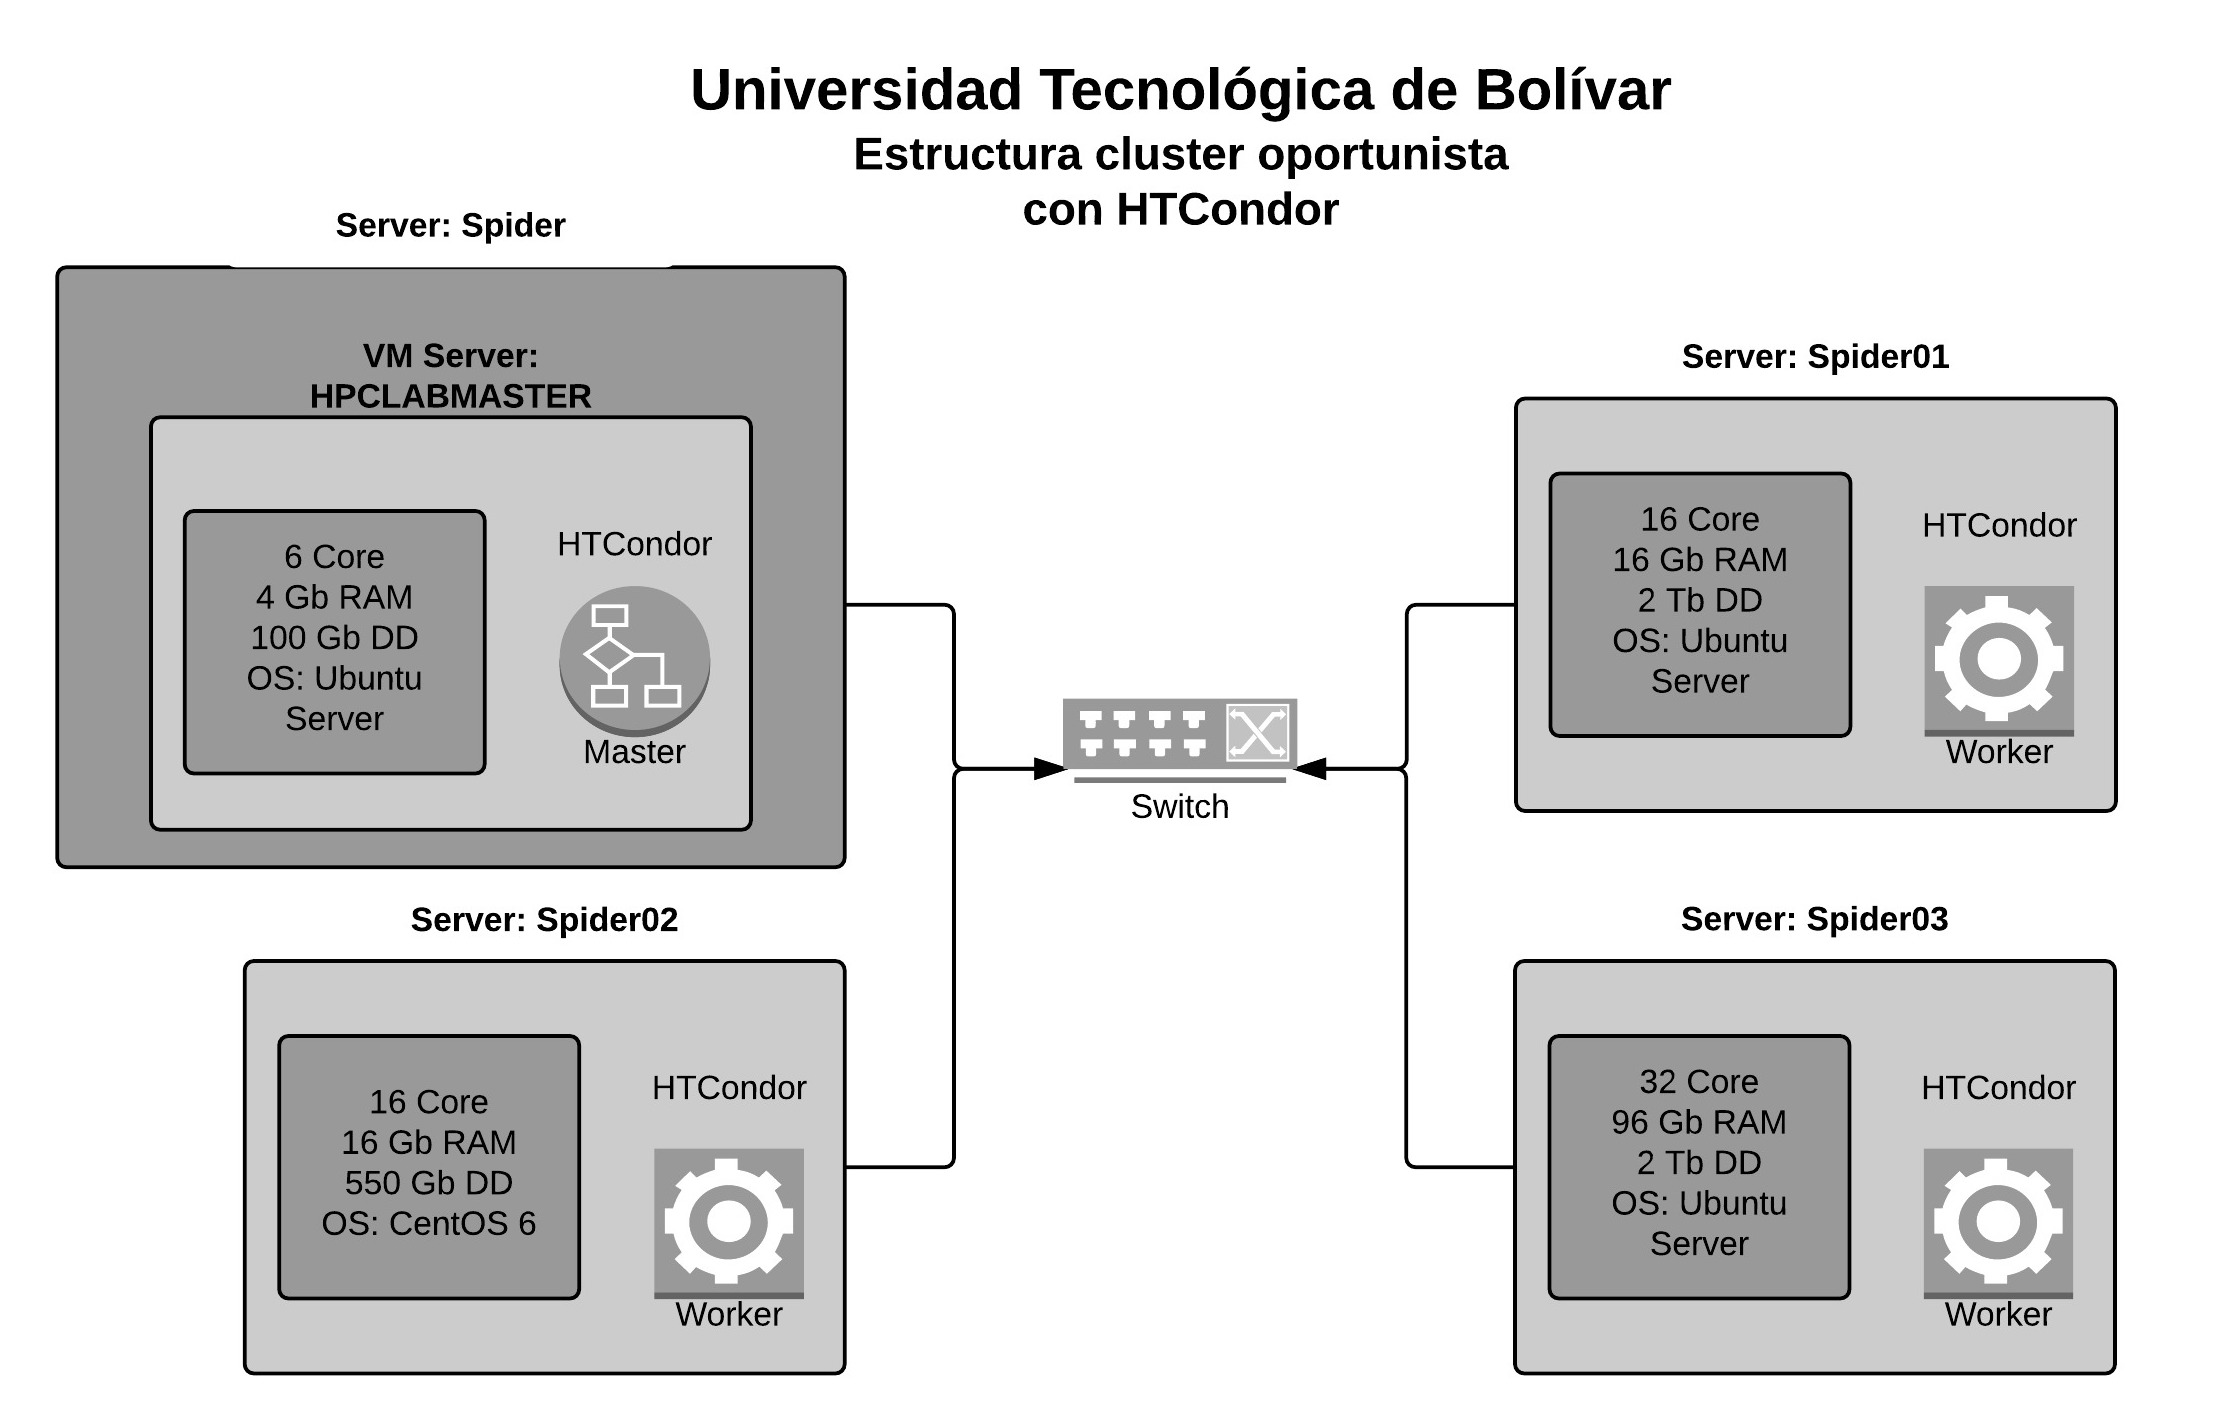
\includegraphics[width=0.95\textwidth]{images/spidercluster.jpeg}
\decoRule
\caption{Estructura HTCondor en la UTB}
\label{fig:UTB_Condor}
\end{figure}
\FloatBarrier

El nodo maestro es una máquina virtual instalada en el servidor físico \mbox{\textbf{Spider}}, esta máquina virtual cuenta con 6 procesadores, 4Gb RAM y 100Gb de espacio en disco para almacenamiento.

\begin{figure}[h]
\centering
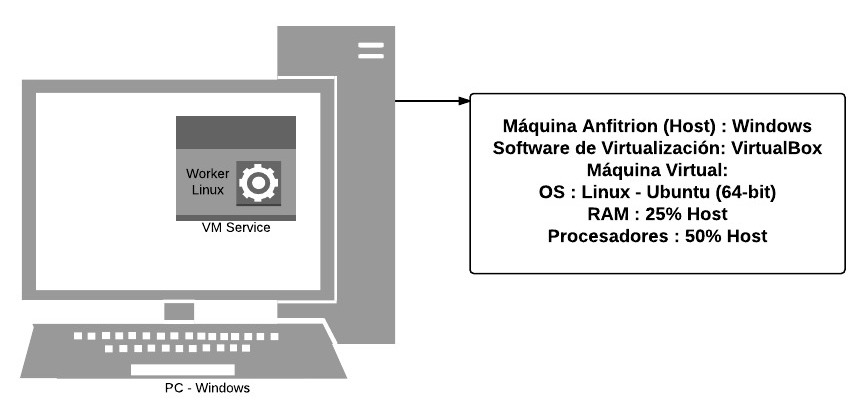
\includegraphics[width=0.95\textwidth]{images/workernode.jpeg}
\decoRule
\caption{Estructura HTCondor en Nodo Windows}
\label{fig:UTB_Condor}
\end{figure}
\FloatBarrier

Ademas de ello cuenta con 6 salones laboratorios que tienen 30 estaciones de trabajo con sistema operativo Windows que son el foco donde se \mbox{implementará} este trabajo.




% Chapter Template

\chapter{Implementación: Despliegue} % Main chapter title

\label{Chapter4} % Change X to a consecutive number; for referencing this chapter elsewhere, use \ref{ChapterX}

%----------------------------------------------------------------------------------------
%	SECTION 1
%----------------------------------------------------------------------------------------

\section{Creación máquina base}
Para poder desplegar las máquinas como servicio en los nodos de trabajo con Windows, primero se crea una máquina virtual para usarla como base.

El gestor de maquinas virtuales utilizado es \textbf{VirtualBox v 5.0.18} que se puede encontrar en la \href{https://www.virtualbox.org/wiki/Downloads}{página principal} o el enlace en la wiki de la universidad \autocite{hpc}.

\subsection*{Sistema Operativo Base}
Como sistema operativo base para el nodo de trabajo, se instala \textbf{Ubuntu 14.04} en su versión de escritorio mínima, el disco de instalación no pesa mas de 50 megas y permite instalar solo los componentes necesarios para la ejecución de y trabajos en segundo plano con la herramienta HTCondor.

Una vez instalado el gestor de máquinas virtuales, se ejecuta y se crea una nueva máquina virtual.
\begin{figure}[h]
\centering
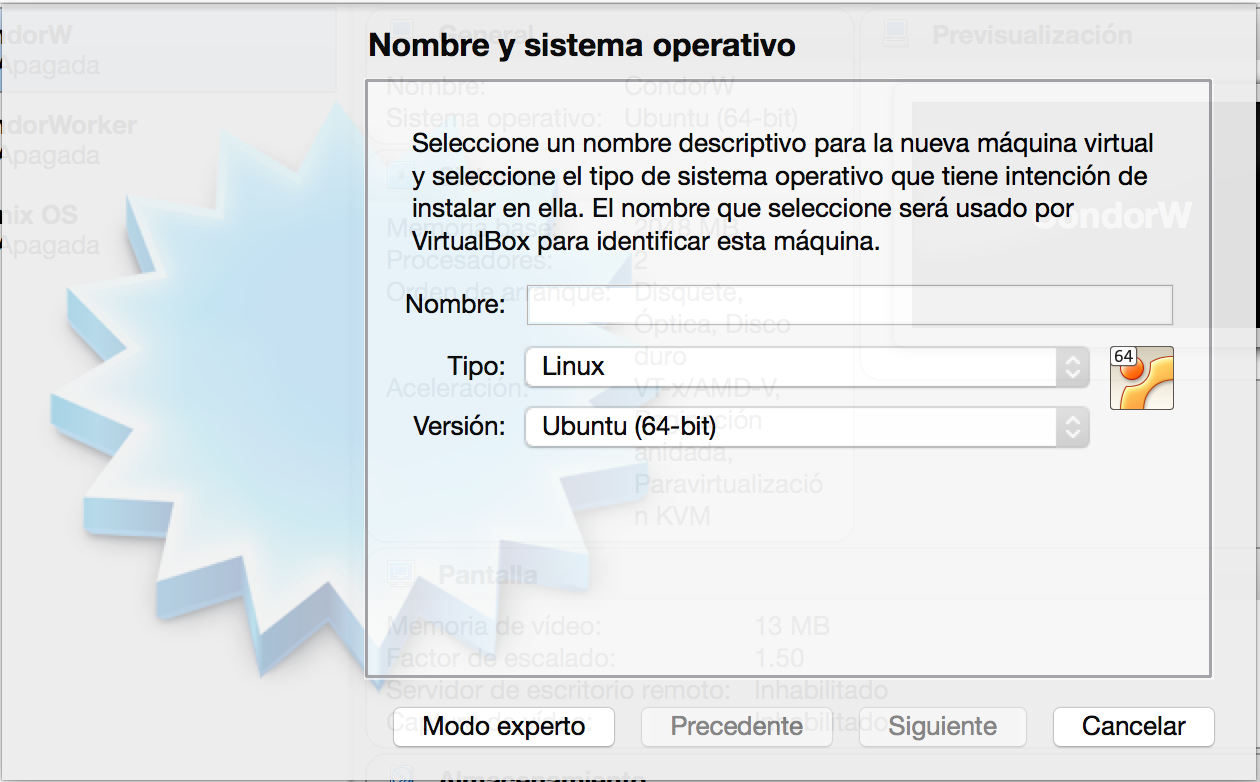
\includegraphics[width=0.7\textwidth]{vbox/newmachine.png}
\decoRule
\caption{Creación máquina virtual}
\label{fig:Nueva máquina}
\end{figure}
\FloatBarrier
Luego de seleccionar un nombre para la máquina y escoger el tipo de sistema operativo y la versión, se selecciona la memoria RAM para la máquina virtual.
\begin{figure}[h]
\centering
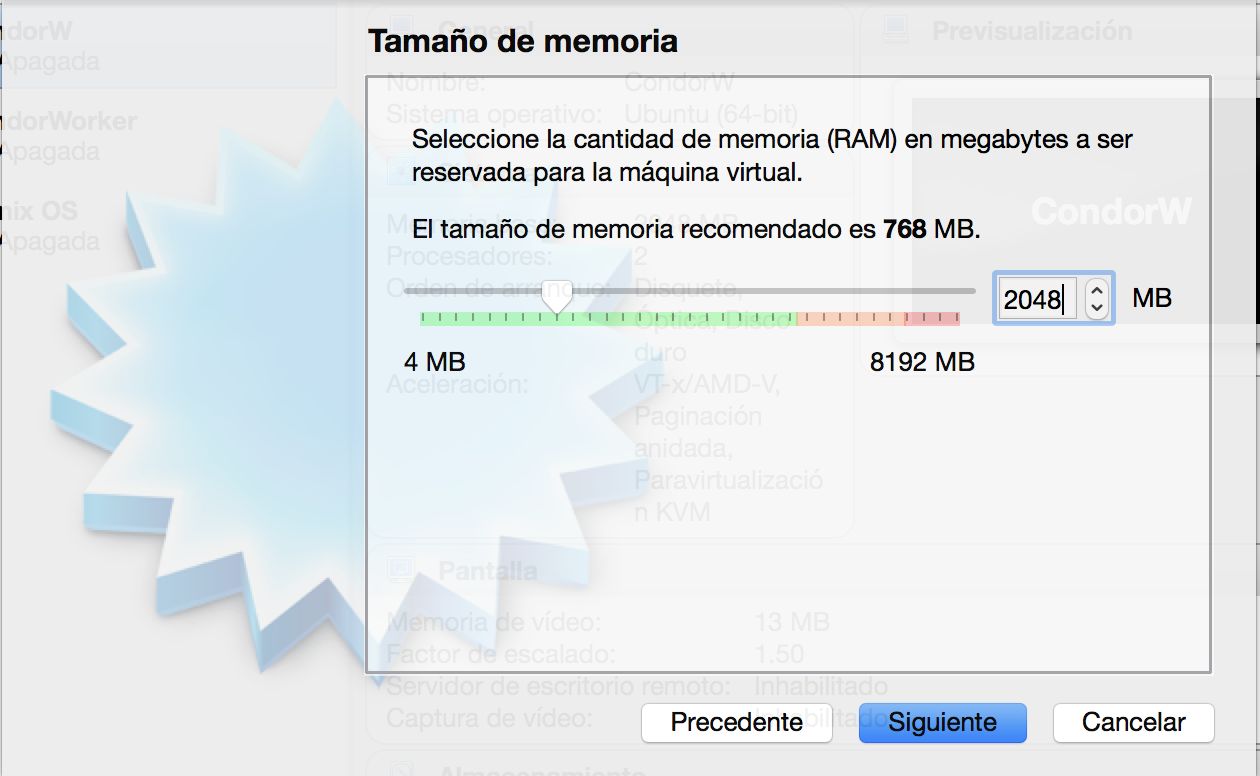
\includegraphics[width=0.7\textwidth]{vbox/memory.png}
\decoRule
\caption{Memoria máquina virtual}
\label{fig:Memoria virtual}
\end{figure}
\FloatBarrier

Se crea un disco virtual que contendrá toda la información de nuestro nodo de trabajo.
\begin{figure}[h]
\centering
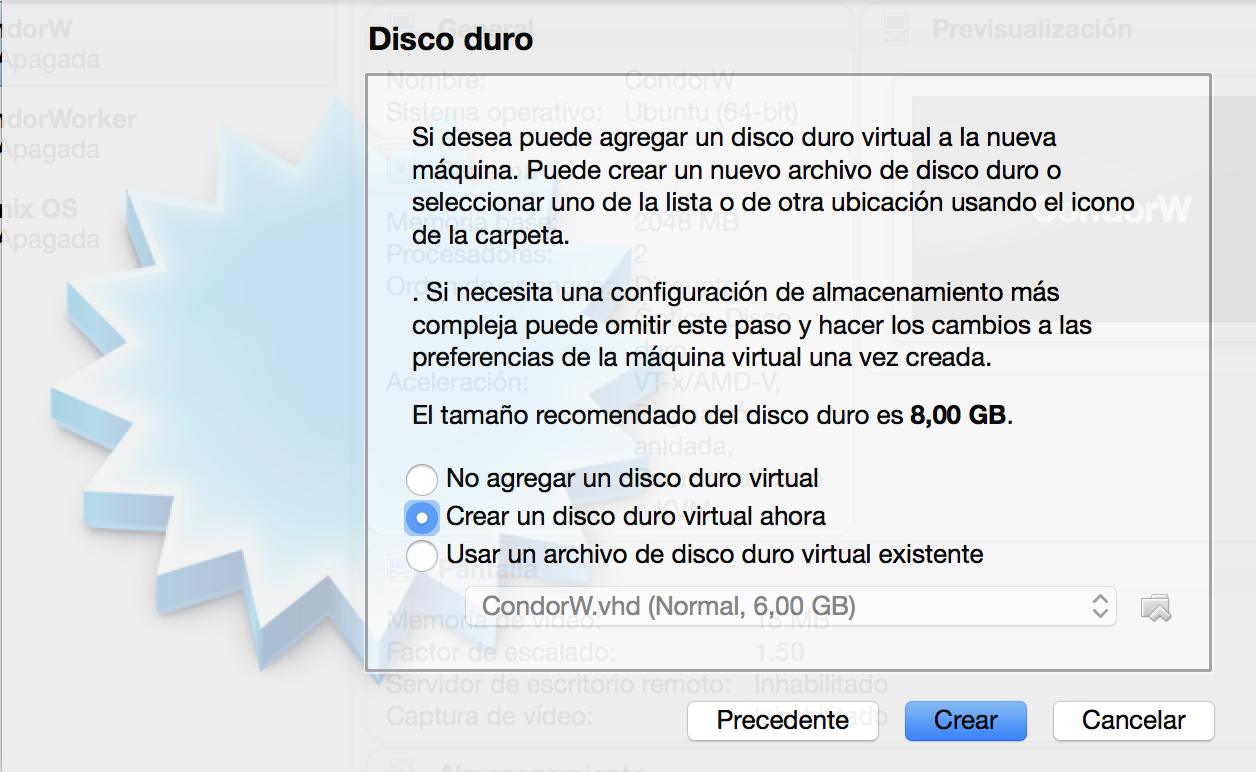
\includegraphics[width=0.7\textwidth]{vbox/virtualdisck.png}
\decoRule
\caption{Creación disco virtual}
\label{fig:Disco virtual}
\end{figure}
\FloatBarrier
El tipo de disco que se crea, en este caso es un Virtual Hard Disck (VHD) con capacidad de 10 GB.

Este espacio sera asignado de manera dinámica, así el tamaño total de la imagen del nodo de trabajo sera mas pequeña y fácil de compartir por la red de la universidad.
\begin{figure}[h]
\centering
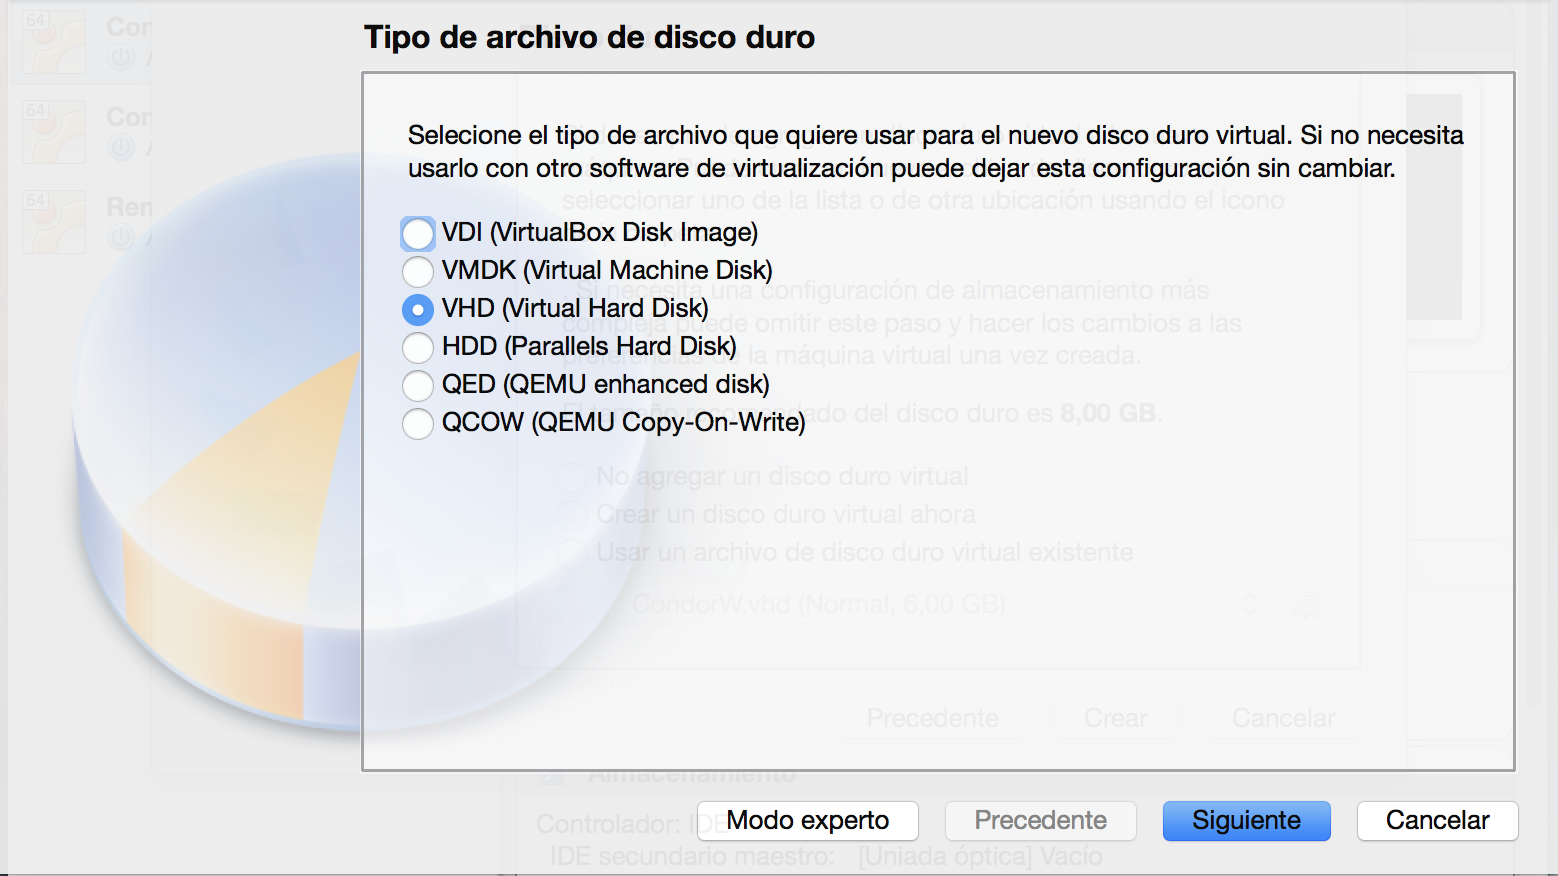
\includegraphics[width=0.7\textwidth]{vbox/vdtype.png}
\decoRule
\caption{Tipo de disco virtual}
\label{fig:hd type}
\end{figure}
\FloatBarrier

El nombre del disco virtual, es por defecto igual al nombre de la máquina virtual.

\begin{figure}[h]
\centering
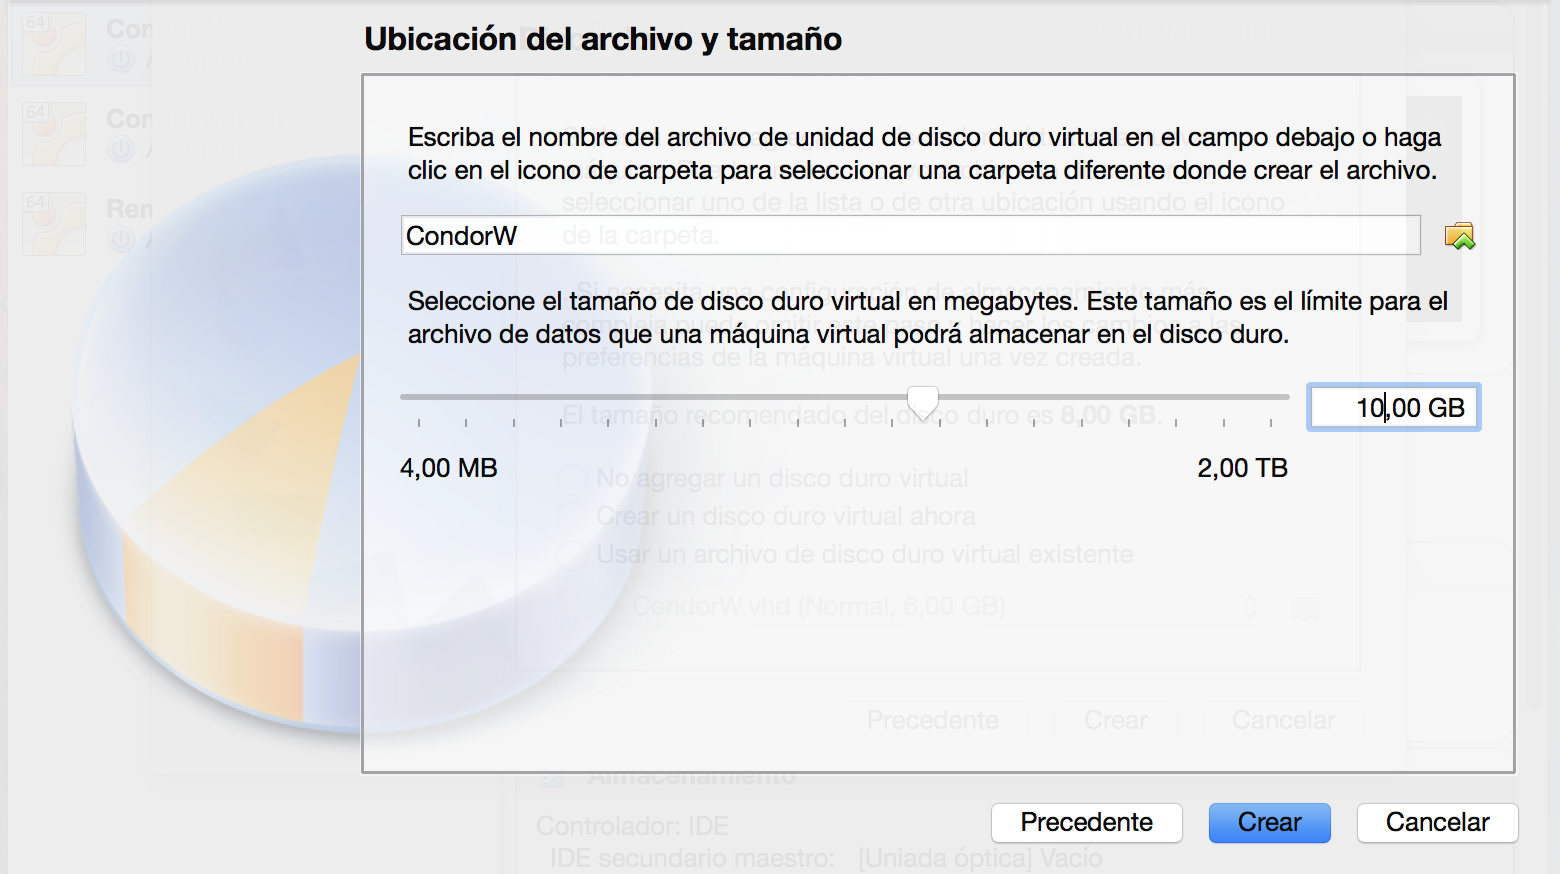
\includegraphics[width=0.7\textwidth]{vbox/vhdsize.png}
\decoRule
\caption{Tamaño disco virtual}
\label{fig:hd size}
\end{figure}
\FloatBarrier
Se le da un tamaño de 10Gb al disco virtual, por lo que se espera trabajar con grandes volúmenes de datos, pero como este disco esta asignado de manera dinámica, el tamaño final es menor al 10Gb, próximo a 3Gb.
\begin{figure}[h]
\centering
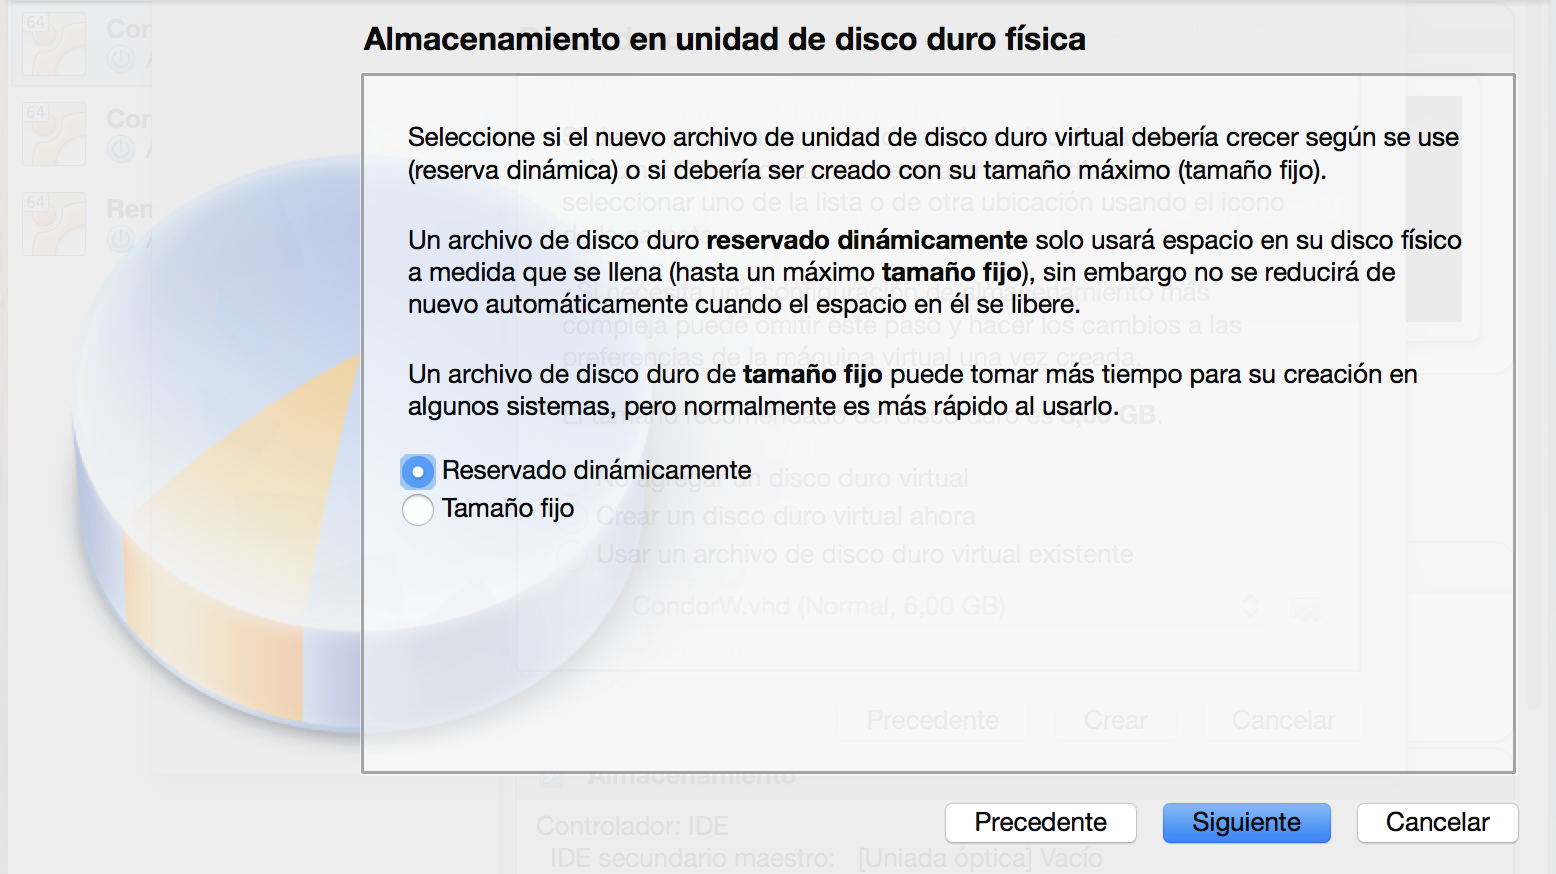
\includegraphics[width=0.7\textwidth]{vbox/dynamicvhd.png}
\decoRule
\caption{Tamaño asignado dinámico}
\label{fig:dynamic size}
\end{figure}
\FloatBarrier

Una vez creado el disco, se procede a montar la imagen del sistema operativo en una unidad virtual para la instalación en nuestra maquina.

Se realiza la instalación de Ubuntu 14.04 Desktop Minimal.

Una vez instalado el sistema operativo, accedemos a la máquina y procedemos a actualizar e instalar los paquetes necesarios para el correcto funcionamiento de HTCondor, El universo de Java, y los scripts necesario para automatizar el nombre de la máquina en el cluster.


\section{Instalación de HTCondor}
El proceso de instalación de HTCondor es realmente sencillo, se hace uso de los repositorios propios de Ubuntu para esto, una vez actualizado el sistema.

\subsection{Paso a paso}
Primero acedemos como usuario \textbf{root} e instalamos HTCondor usando el comando:

\textbf{\textit{apt-get install htcondor}}

Nos mostrará una lista de dependencias que se deben instalar para el correcto funcionamiento de la herramienta.

\begin{figure}[h]
\centering
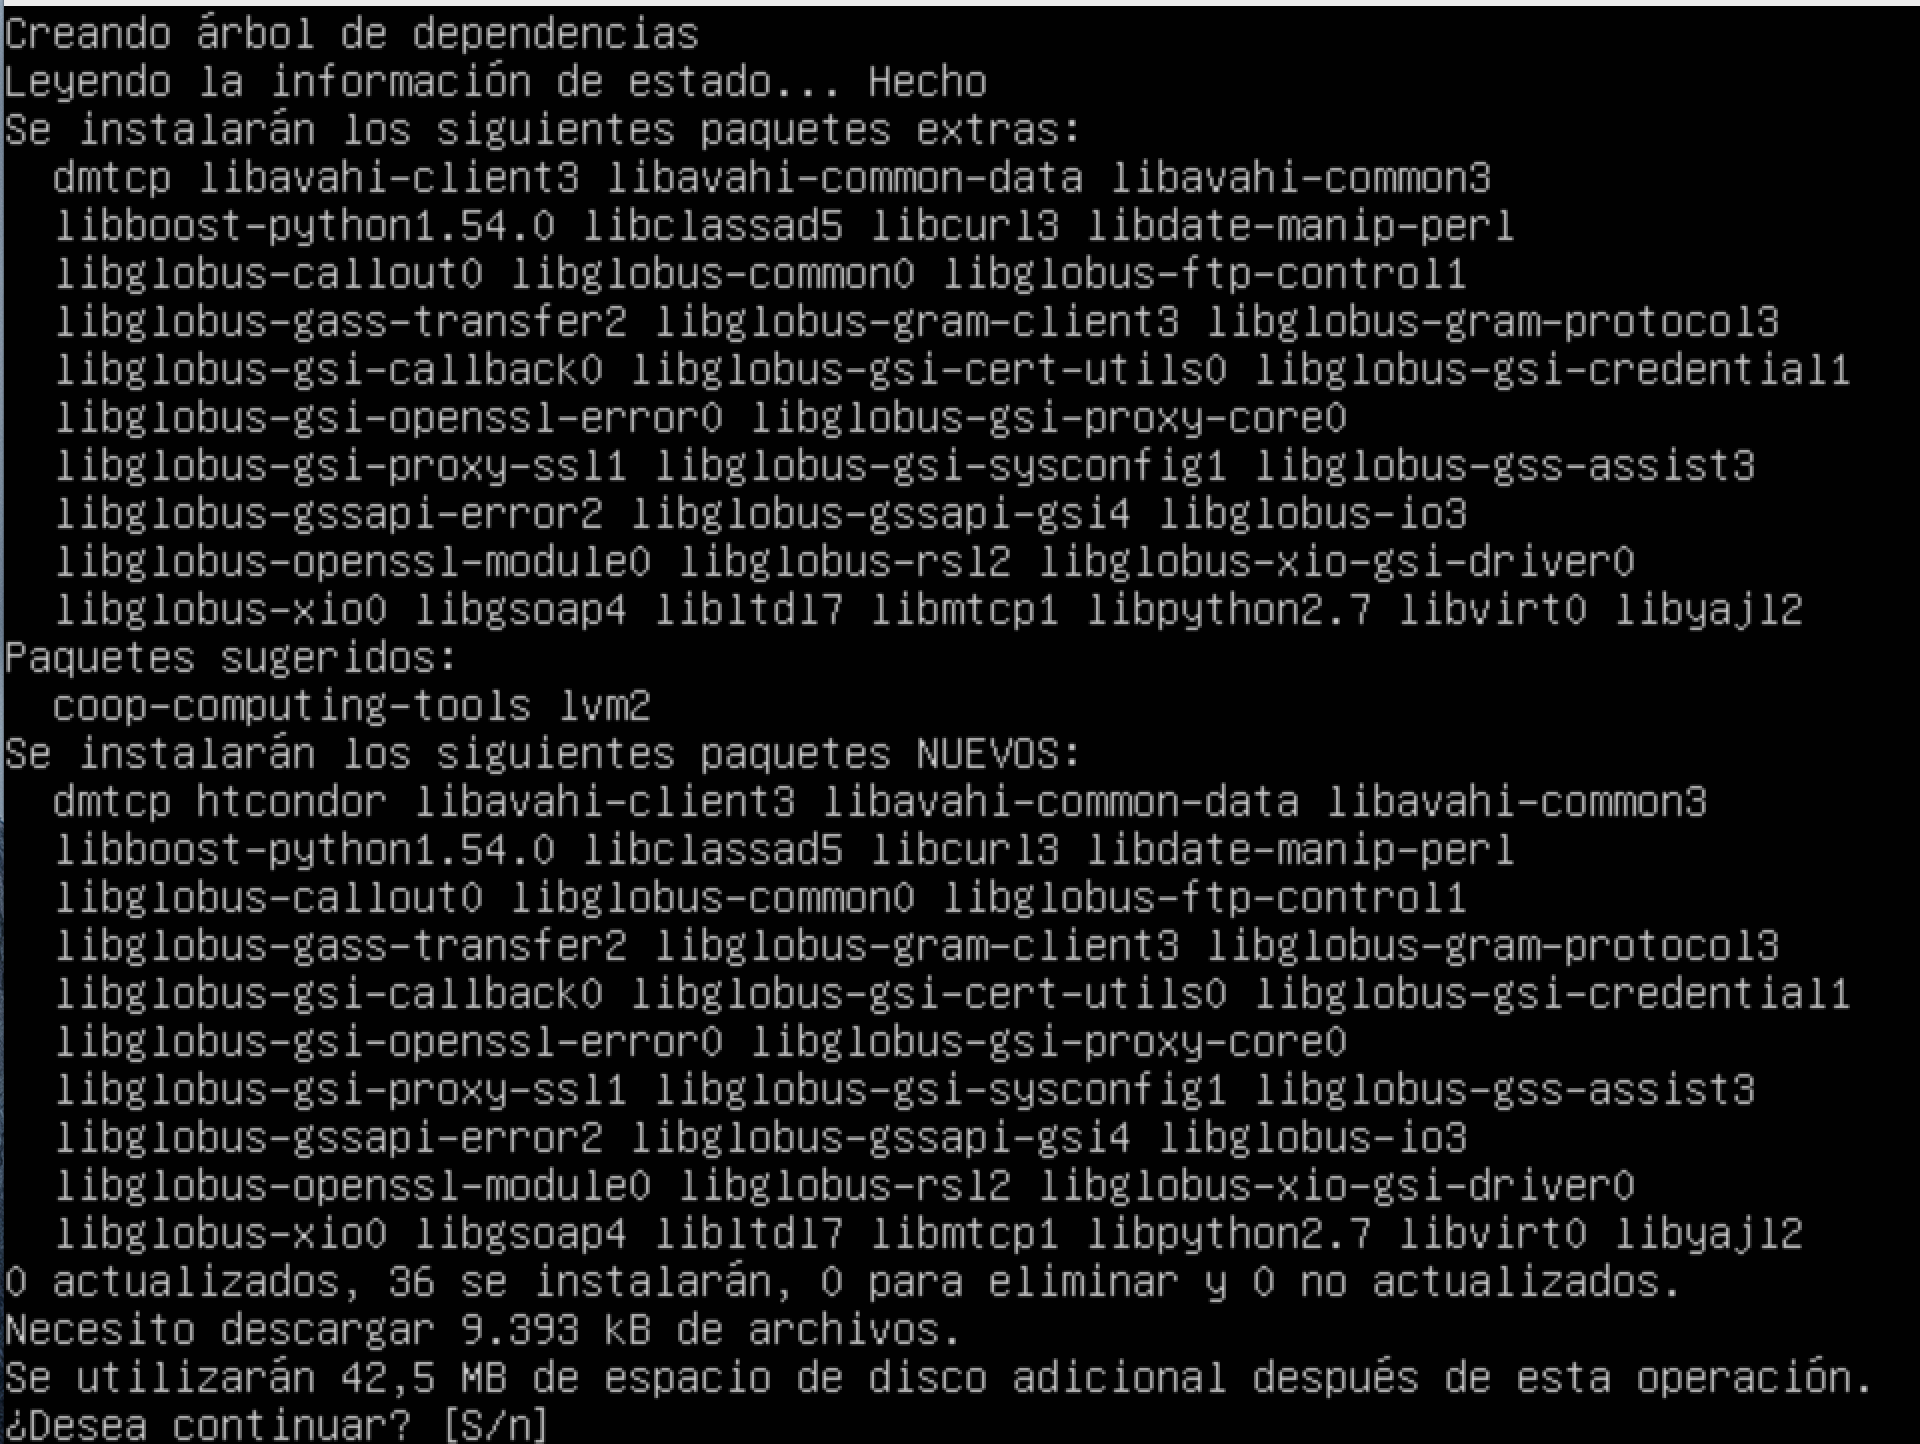
\includegraphics[width=0.8\textwidth]{Figures/dependency.png}
\decoRule
\caption{Dependencias necesarias para HTCondor}
\label{fig:htcondor dependency}
\end{figure}
\FloatBarrier

Luego nos pedirá si deseamos modificar los parámetros de configuración inicial de condor, le decimos que no, ya que el archivo de configuración lo editaremos mas adelante.

\begin{figure}[h]
\centering
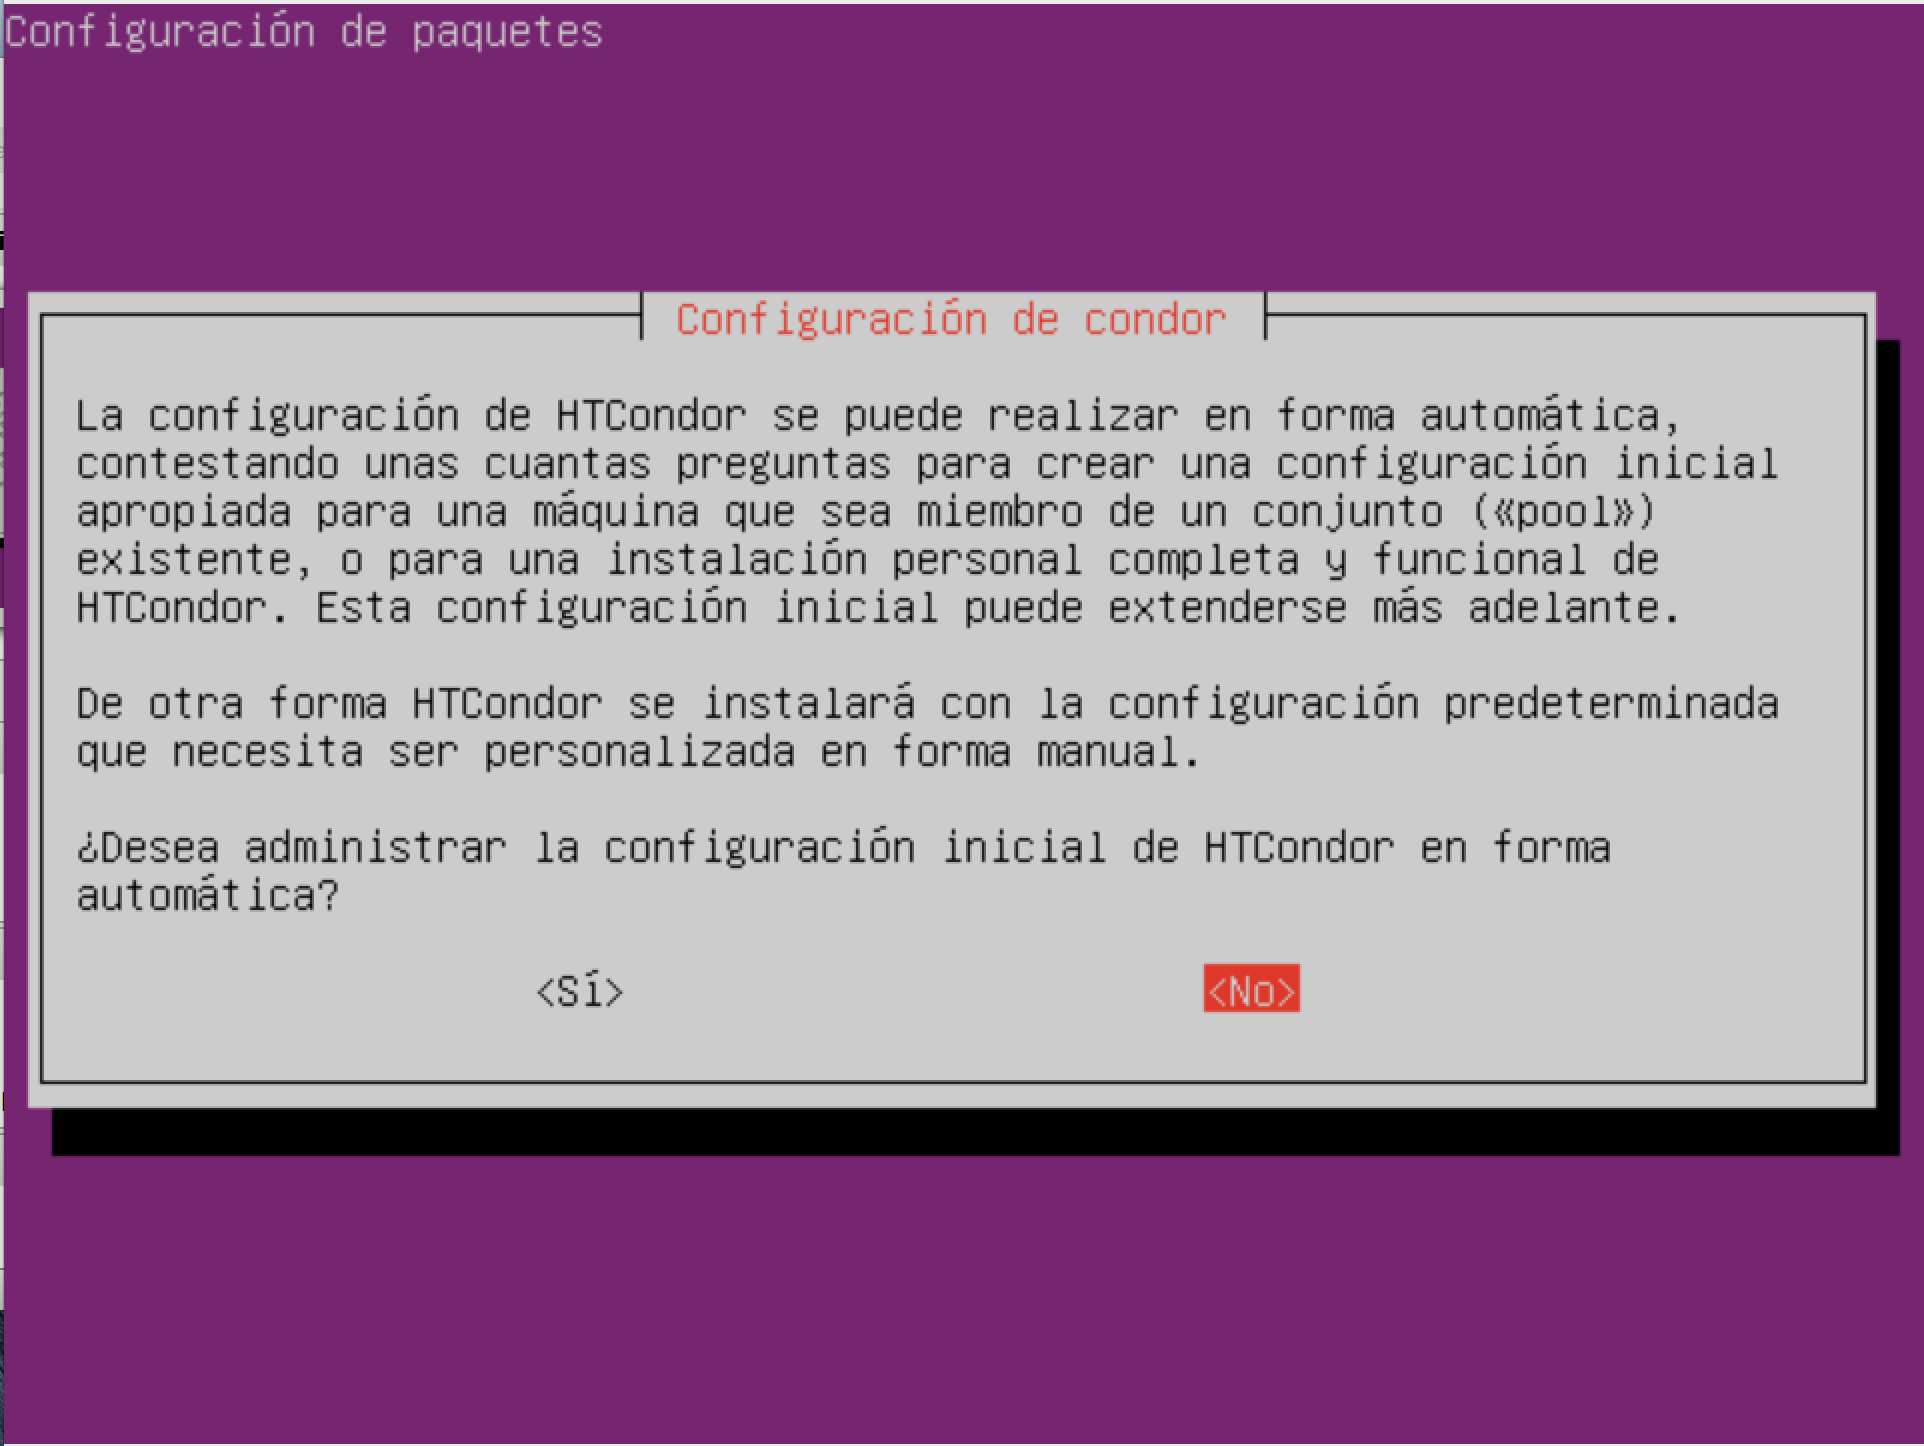
\includegraphics[width=0.8\textwidth]{Figures/preconf.png}
\decoRule
\caption{Configuración inicial}
\label{fig:htcondor pre-conf}
\end{figure}
\FloatBarrier

Verificamos que HTcondor esta correctamente instalado y ejecutándose usando el comando:

\textbf{\textit{ps aux | grep condor}}

\begin{figure}[h]
\centering
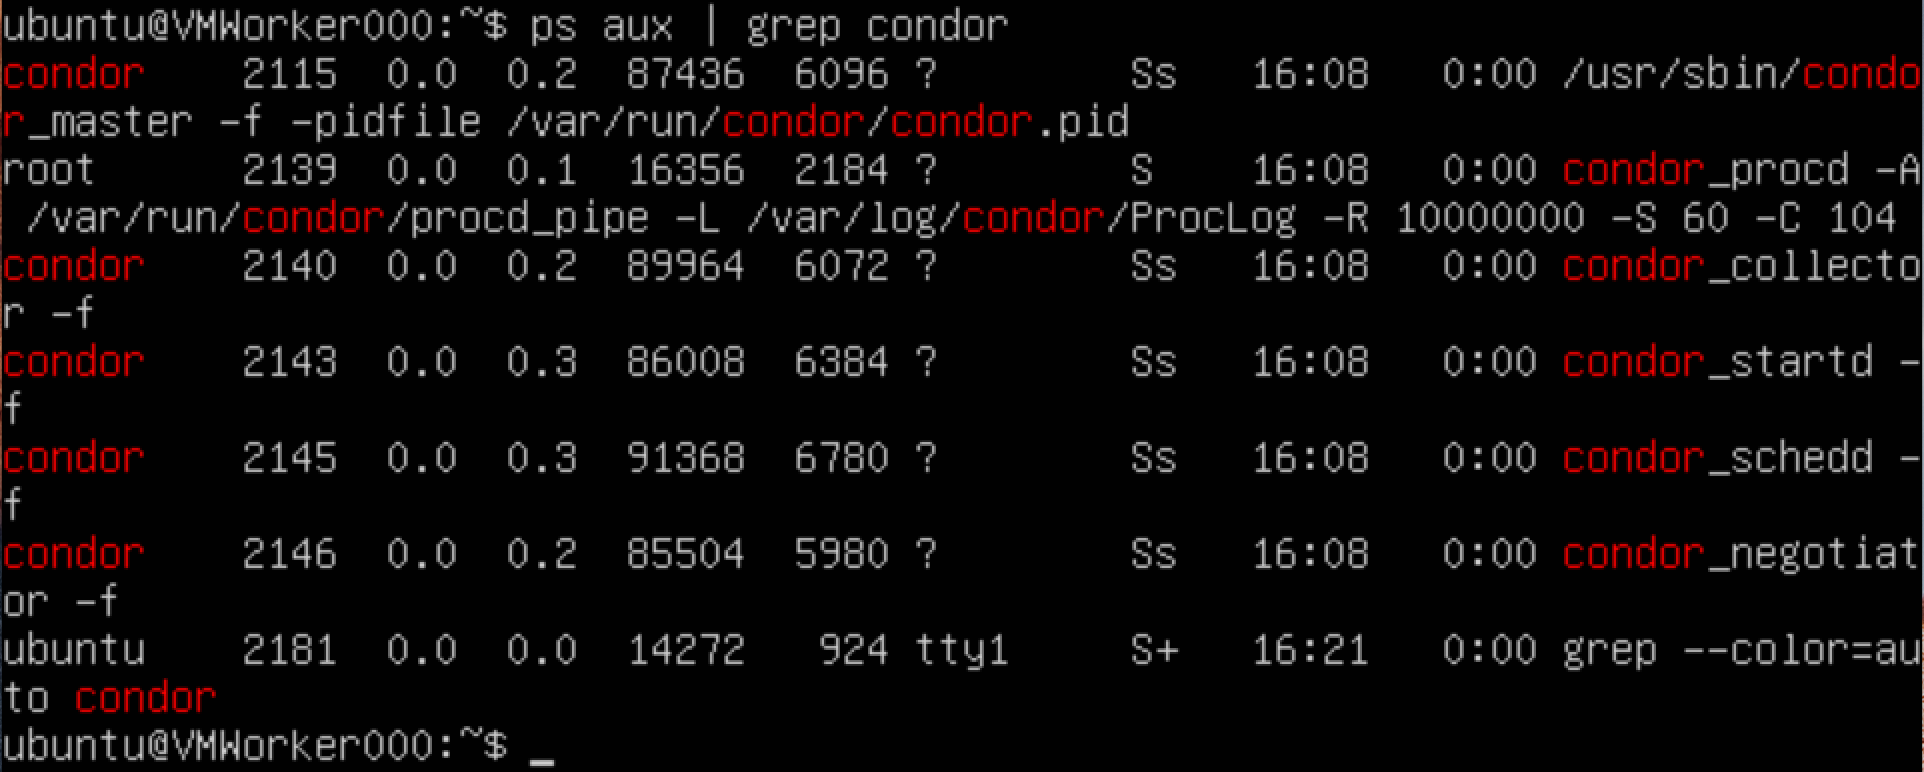
\includegraphics[width=0.8\textwidth]{Figures/running.png}
\decoRule
\caption{HTCondor activo en el sistema}
\label{fig:htcondor pre-conf}
\end{figure}
\FloatBarrier

\section{Instalación de Java}

Luego de la instalación de HTCondor, se procede con la instalación de Java en el sistema, para ello se usa un PPA con la información reciente de Java versión 8.

para ello primero instalamos la herramienta de manejo de PPA

\textbf{\textit{apt-get install software-properties-common}}

y luego agregamos el PPA correspondiente a Java.

\textbf{sudo add-apt-repository ppa:webupd8team/java}

\begin{figure}[h]
\centering
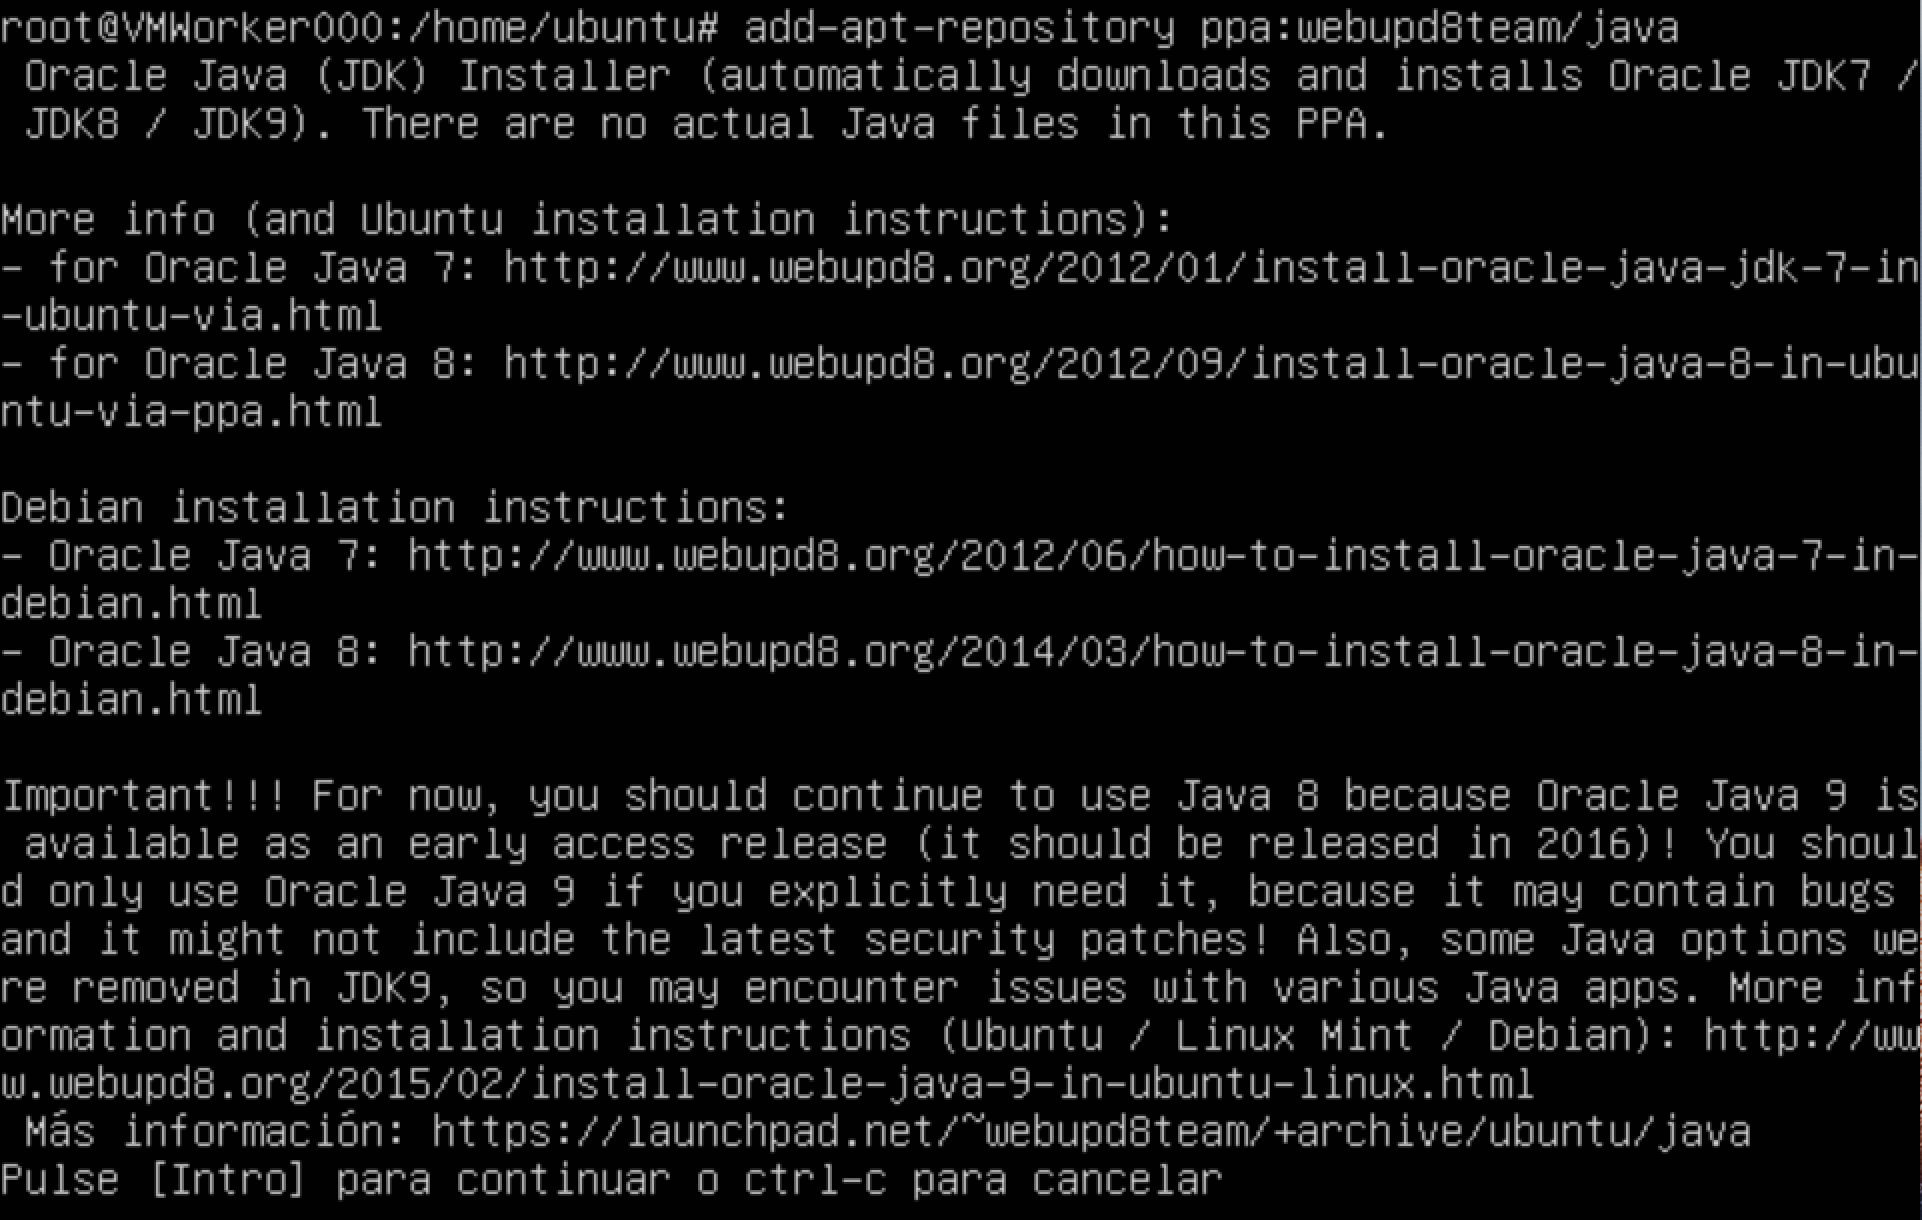
\includegraphics[width=0.8\textwidth]{Figures/ppajava.png}
\decoRule
\caption{PPA Java}
\label{fig:ppa java}
\end{figure}
\FloatBarrier

\begin{figure}[h]
\centering
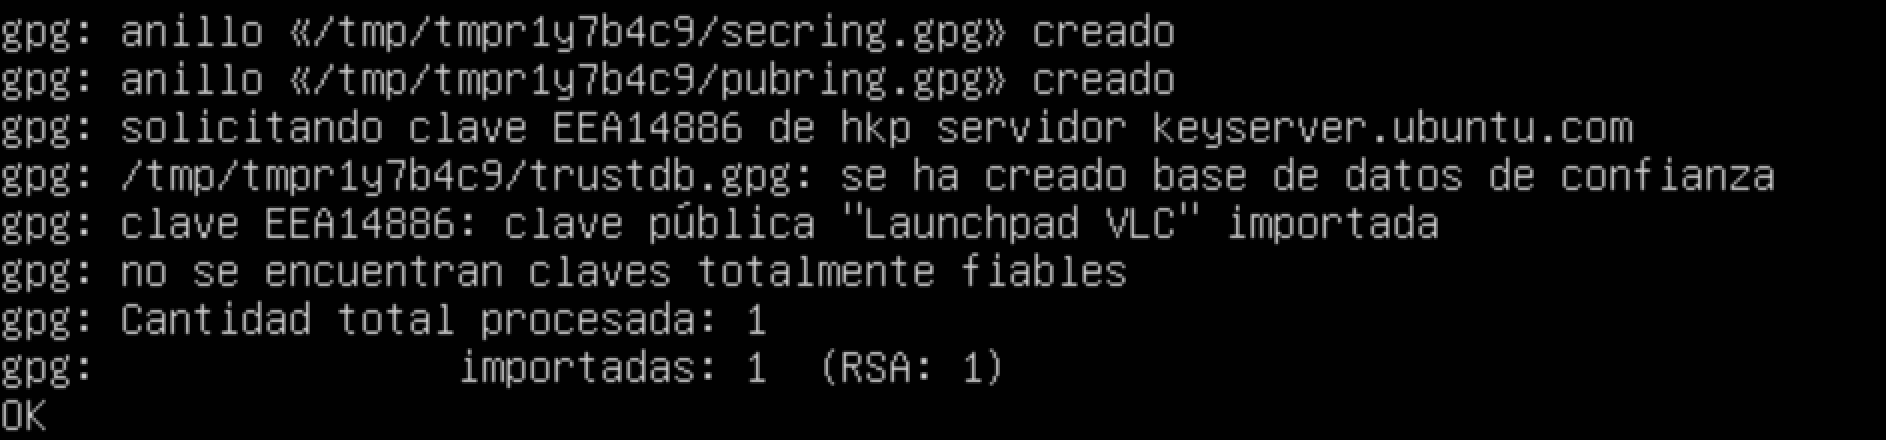
\includegraphics[width=0.8\textwidth]{Figures/ppajavaok.png}
\decoRule
\caption{PPA Java instalado}
\label{fig:ppa java aceptación}
\end{figure}
\FloatBarrier
Luego se actualiza la lista de paquetes del sistema usando el comando:

\textbf{sudo apt-get update}

Y se procede a instalar Java 8.

\textbf{sudo apt-get install oracle-java8-installer}
\begin{figure}[h]
\centering
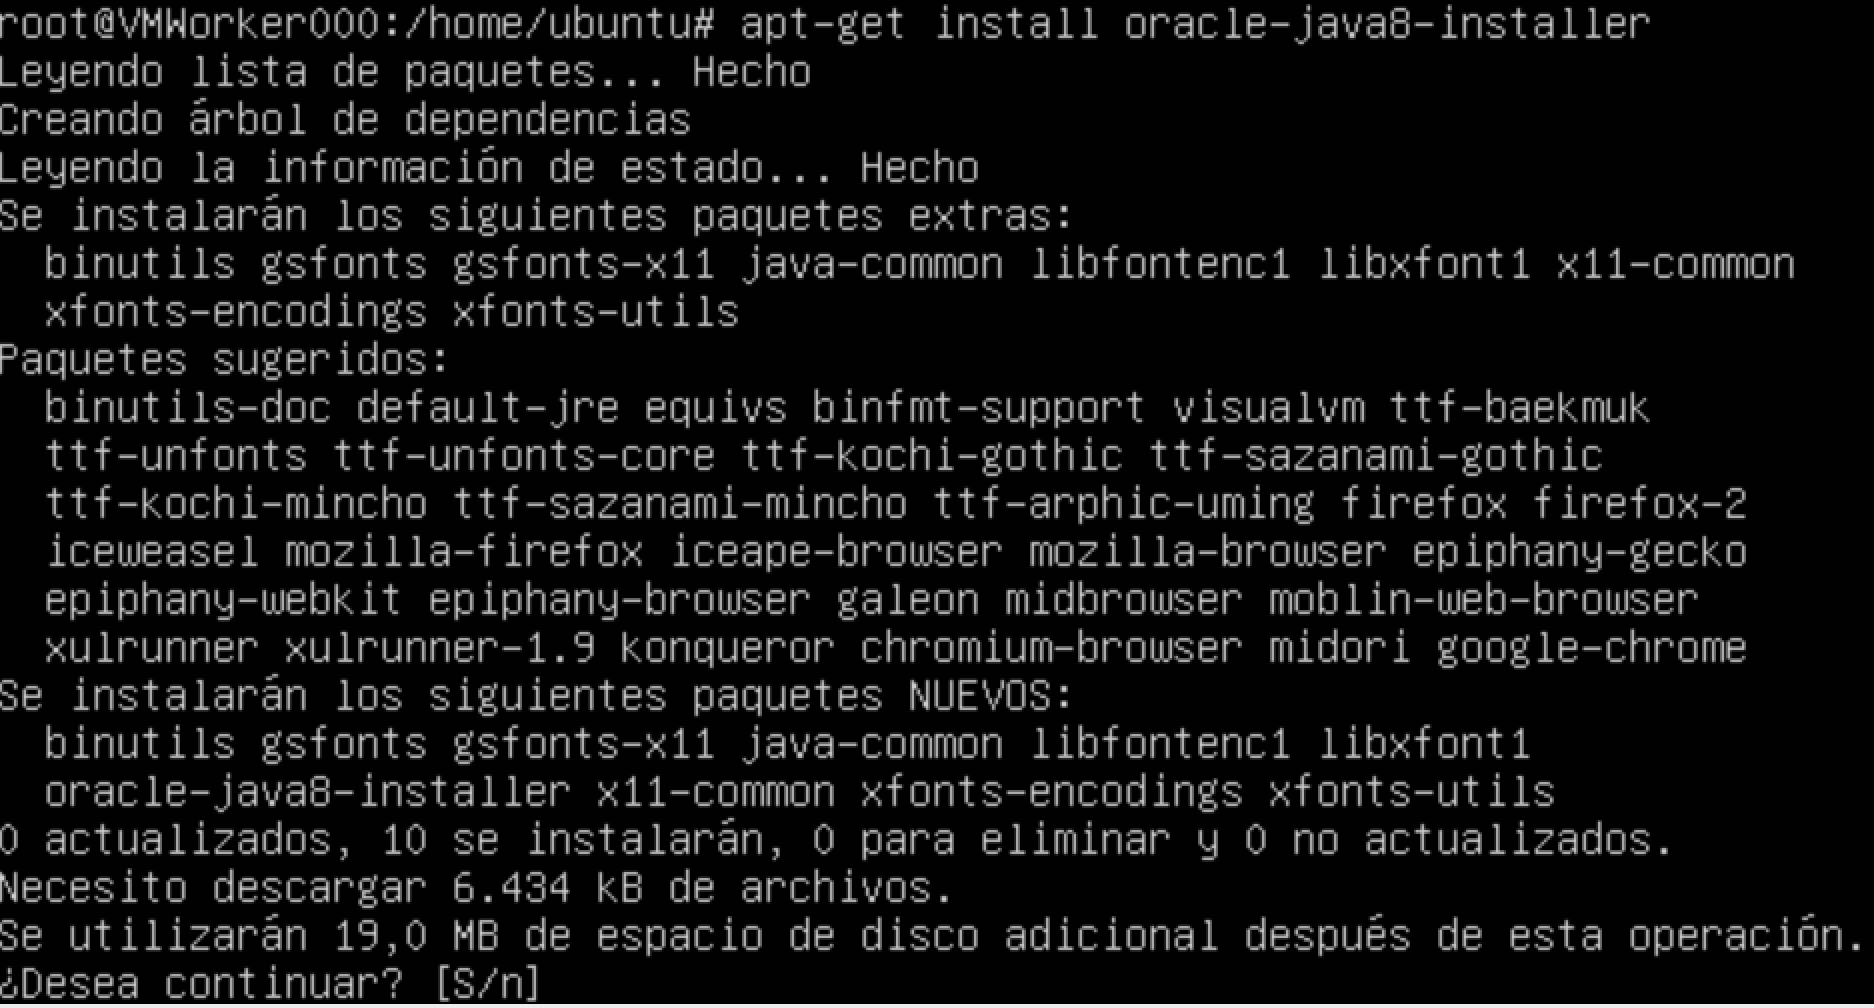
\includegraphics[width=0.8\textwidth]{Figures/javainstall.png}
\decoRule
\caption{Comando instalación de Java}
\label{fig:Java install command}
\end{figure}
\FloatBarrier

Se aceptan luego los términos y condiciones de Java 8.

\begin{figure}[h]
\centering
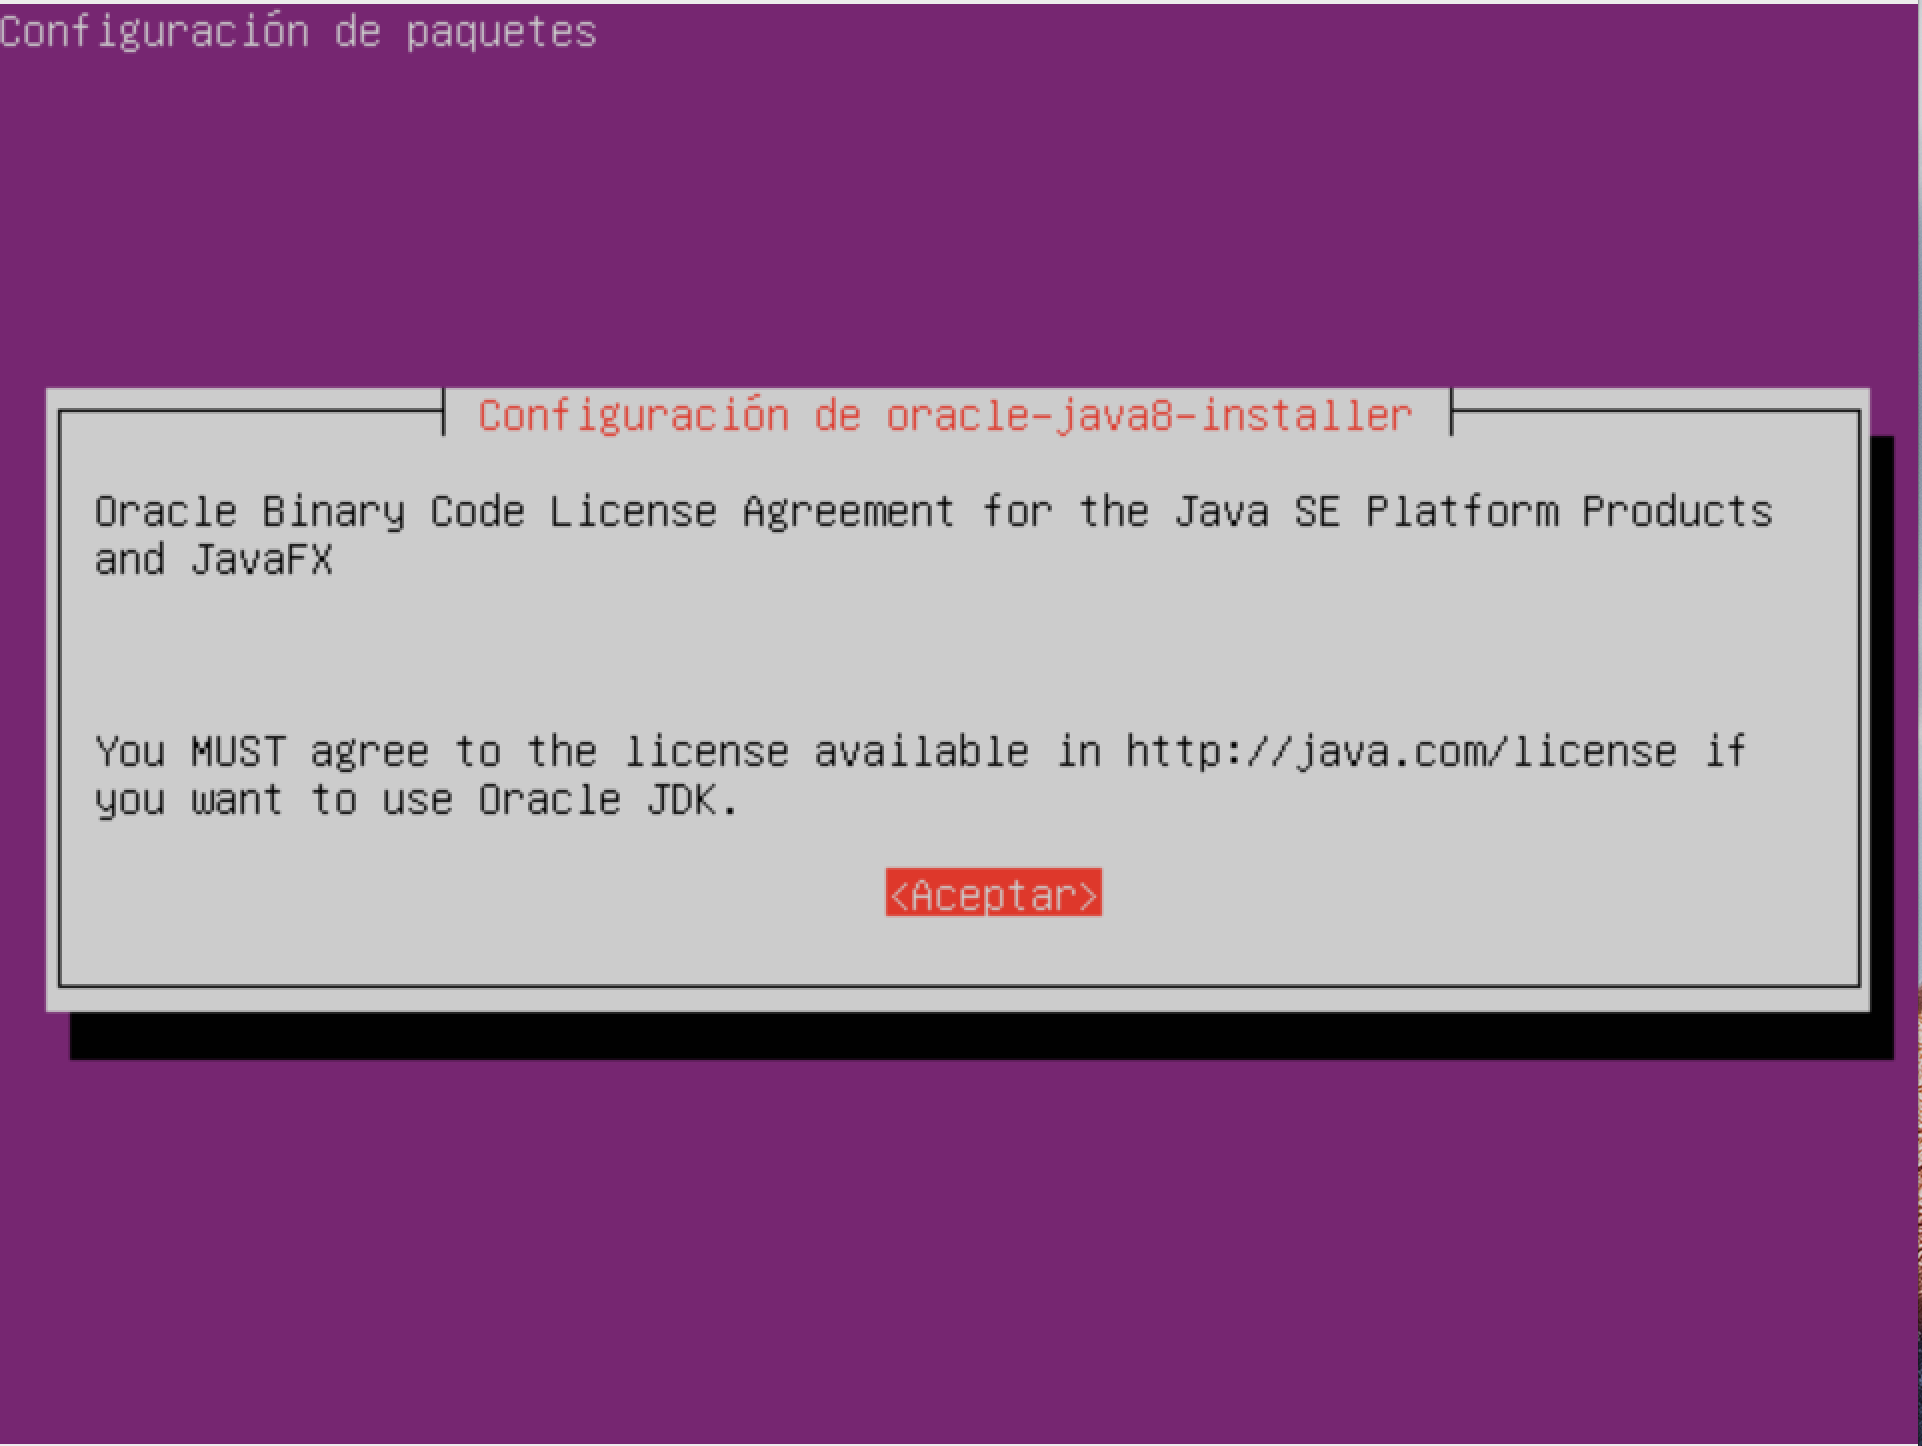
\includegraphics[width=0.8\textwidth]{Figures/javaagree.png}
\decoRule
\caption{Aceptación de instalación}
\label{fig:Java agree}
\end{figure}
\FloatBarrier

Confirmamos que java este instalado correctamente y vemos la versión del mismo con el comando:

\textbf{ java -version}

\begin{figure}[h]
\centering
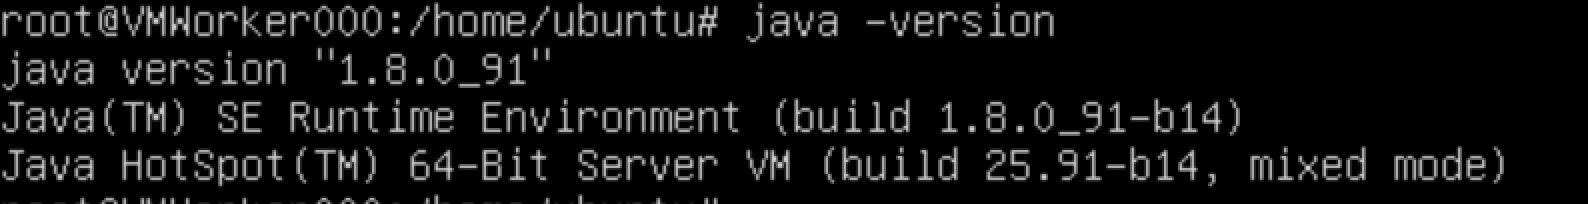
\includegraphics[width=0.8\textwidth]{Figures/javaversion.png}
\decoRule
\caption{Instalación finalizada}
\label{fig:Java version}
\end{figure}
\FloatBarrier

\section{Instalación de GCC}
Una vez instalado Java, procedemos a la instalación de las librerías y compiladores de C y C++ (\textbf{gcc}).

\textbf{apt-get install gcc}

\begin{figure}[h]
\centering
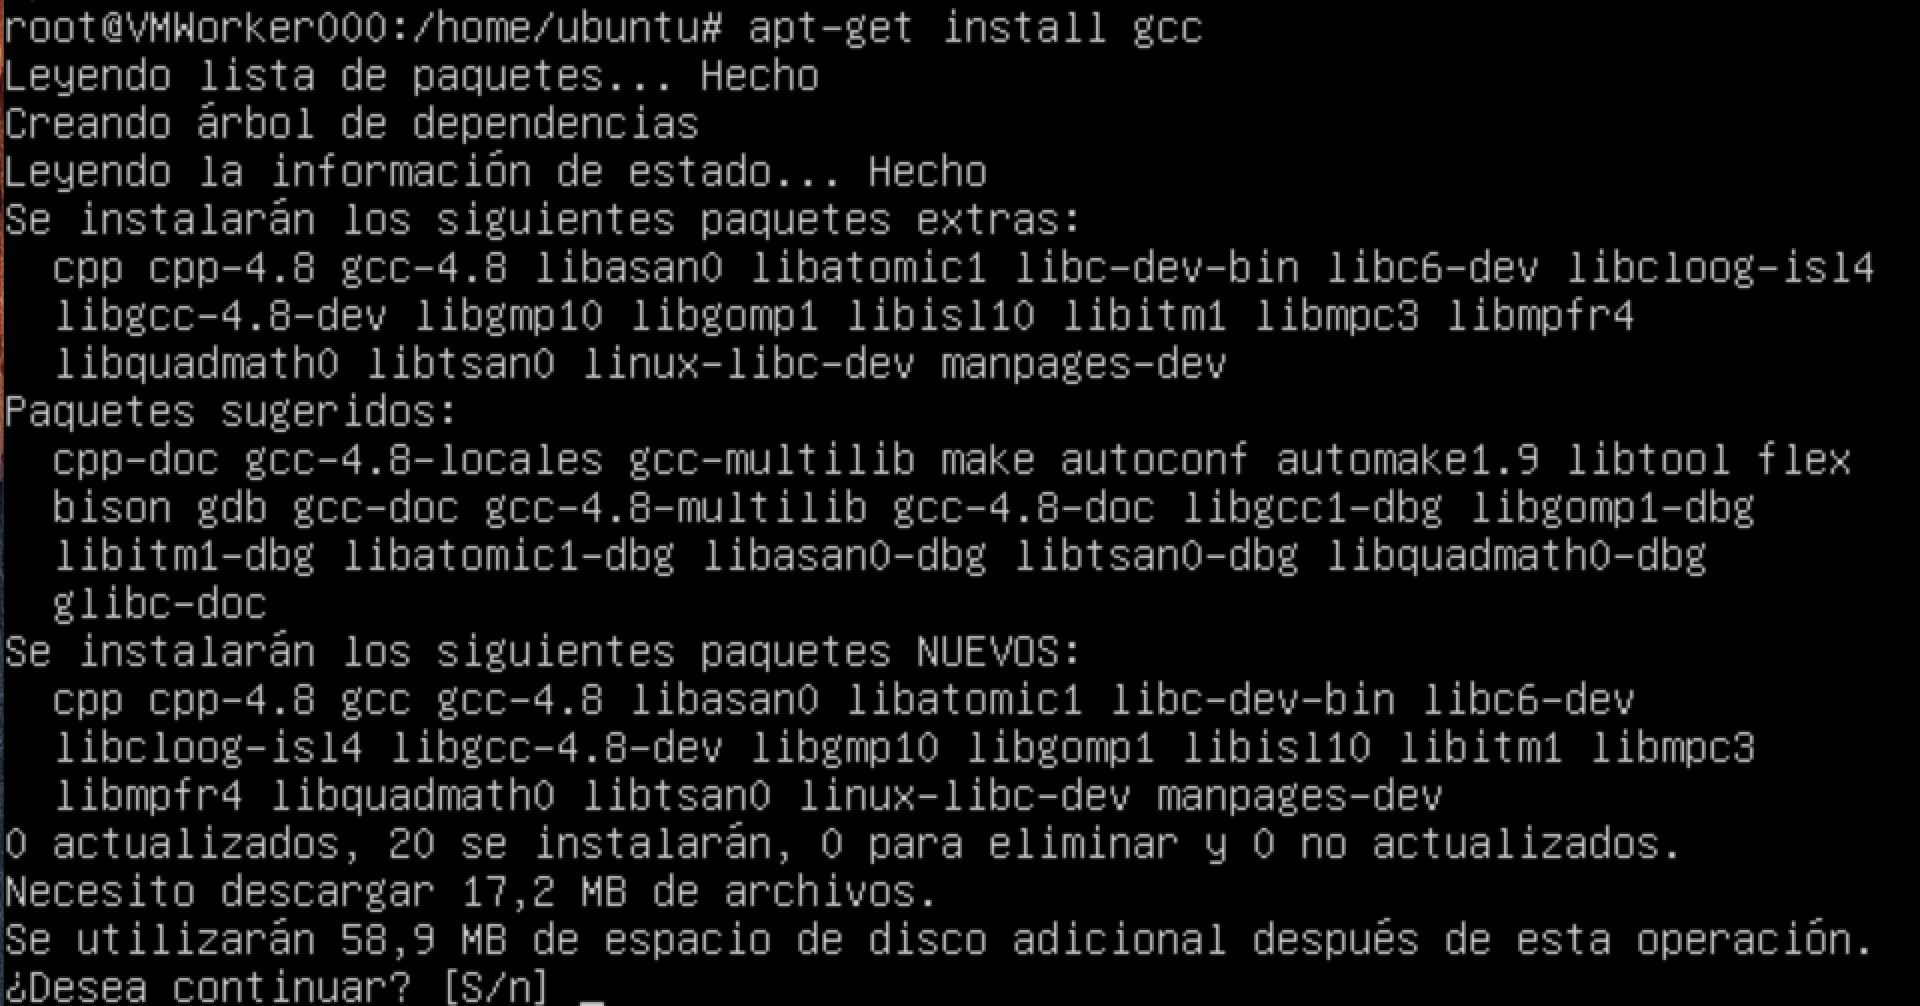
\includegraphics[width=0.8\textwidth]{Figures/gccinstall.png}
\decoRule
\caption{Instalación de gcc}
\label{fig:GCC install}
\end{figure}
\FloatBarrier
Verificamos la instalación de gcc con el comando:

\textbf{which gcc}

\begin{figure}[h]
\centering
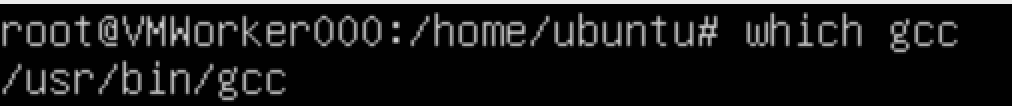
\includegraphics[width=0.8\textwidth]{Figures/gccok.png}
\decoRule
\caption{gcc instalado}
\label{fig:GCC ready}
\end{figure}
\FloatBarrier

En la carpeta del usuario, hay un ejemplo un programa en c que corre el famoso Hola mundo! ( Hola, UTB! ) que muestra el funcionamiento de las librerías de c y c++

\begin{figure}[h]
\centering
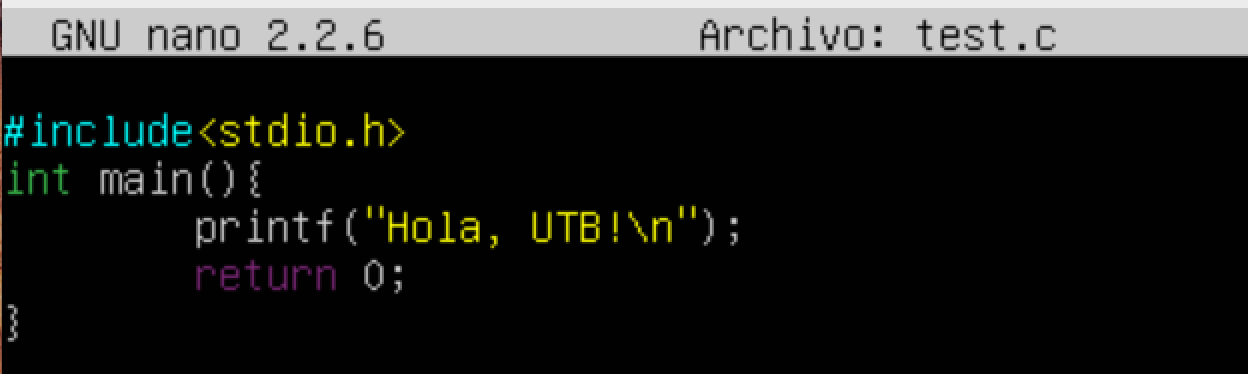
\includegraphics[width=0.8\textwidth]{Figures/pruebagcc.png}
\decoRule
\caption{Código de prueba gcc}
\label{fig:GCC program}
\end{figure}
\FloatBarrier

\begin{figure}[h]
\centering
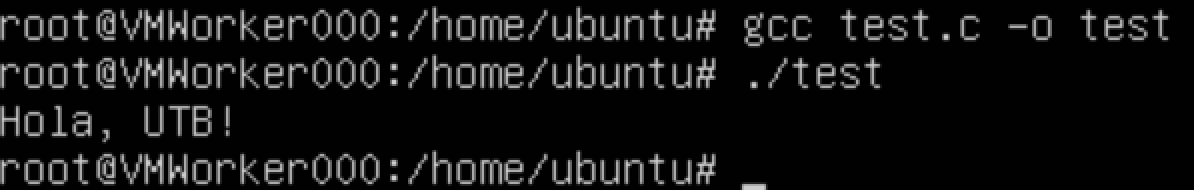
\includegraphics[width=0.8\textwidth]{Figures/testgccok.png}
\decoRule
\caption{gcc prueba de ejecución}
\label{fig:GCC test ok}
\end{figure}
\FloatBarrier

Uva vez ya configuradas las herramientas se procede a configurar HTCondor para la ejecución de tareas.
%-------------------------------------------------------- 
\chapter{Implementación: Configuración} % Main chapter title

\label{Chapter5} 

%--------------------------------------------------------
\section{Configuración de HTCondor}

Se deben tener en claro dos cosa a la hora de configurar una máquina para el uso de HTCondor, si esta sera un nodo de trabajo, o sera el nodo maestro que se encarga de enviar las tareas que se llevaran a cabo.

Dado que este trabajo esta basado en un cluster oportunista, se centra en la configuración de los nodos que realizan los trabajos ("workers").

\subsection{Configuración inicial}

Una vez terminada la instalación de las dependencias necesarias, se procede con la creación y modificación del archivo que contendrá la configuración con la cual iniciará el nodo de trabajo. 

\textbf{Para tener en cuenta:} Los cambios que se realizan a continuación se hacen como usuario \textbf{root} que es quien tiene los permisos para modificar estos archivos.

Primero crearemos el archivo que contendrá la configuración en la ruta:

\textit{/etc/condor/config.d/}

y le colocaremos como nombre \textbf{spider.conf}

\textbf{cd /etc/condor/config.d/}

\textbf{touch spider.conf}

Abrimos el archivo \textbf{spider.conf} y procedemos a editarlo

\begin{lstlisting}
UID_DOMAIN = unitecnologica.edu.co
####################################################################
# Nombre legible para el Condor pool
COLLECTOR_NAME = "Mi cluster en $(UID_DOMAIN)"
# Permisos de escritura
ALLOW_WRITE = *.$(UID_DOMAIN)
CONDOR_ADMIN = root@$(FULL_HOSTNAME)
####################################################################
# The following should be the full name of the head node
CONDOR_HOST = 172.16.9.100
####################################################################
# Rango de puertos usados por condor 
# se deben abrir estos puertos en el firewall de ser necesario
IN_HIGHPORT = 9999
IN_LOWPORT = 9000
####################################################################
# This is to enforce password authentication
SEC_DAEMON_AUTHENTICATION = required
SEC_DAEMON_AUTHENTICATION_METHODS = password
SEC_CLIENT_AUTHENTICATION_METHODS = password,fs,gsi,kerberos
SEC_PASSWORD_FILE = /etc/condor/password
ALLOW_DAEMON = condor_pool@*
##  Sets how often the condor_negotiator starts a negotiation cycle
##  for negotiator and schedd).
#  Defined in seconds and defaults to 60 (1 minute), default is 300.
NEGOTIATOR_INTERVAL = 20
##  Scheduling parameters for the startd
TRUST_UID_DOMAIN = TRUE
####################################################################
# start as available and do not suspend, preempt or kill
START = True
SUSPEND = False
CONTINUE = False
PREEMPT = False
KILL = False
WANT_SUSPEND = True
WANT_VACATE = True
####################################################################
#Como es worker, solo debe iniciar dos demonios
DAEMON_LIST = MASTER, STARTD
SOFT_UID_DOMAIN = TRUE
\end{lstlisting} 


\subsection{Seguridad y autenticación}
Para el manejo de la seguridad en el envío de trabajos y como se comunican las maquinas se colocan los  parámetros, y se agrega la clave del nodo maestro, que es la clave del pool de máquinas.

Para ello, se reinicia el servicio de condor, y luego se ejecuta el siguiente comando

\begin{lstlisting}
condor_store_cred -c add
\end{lstlisting}
Para ingresar la clave previamente compartida del nodo maestro. 

\begin{figure}[h]
\centering
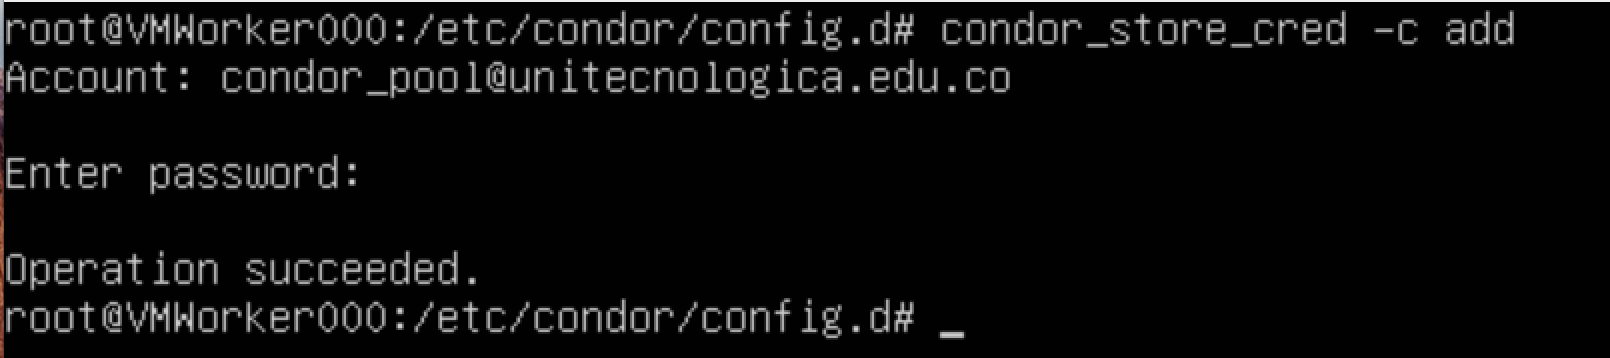
\includegraphics[width=0.8\textwidth]{Figures/pswrdok.png}
\decoRule
\caption{Contraseña compartida aceptada}
\label{fig:condor creed}
\end{figure}
\FloatBarrier

Vemos que la maquina ya lista sus recursos en el pool de condor, la captura fue tomada desde uno de los servidores físicos del plantel, que ya hace parte del cluster.

el comando para listar los recursos disponibles en el pool es:
\begin{lstlisting}
condor_status
\end{lstlisting}

\begin{figure}[h]
\centering
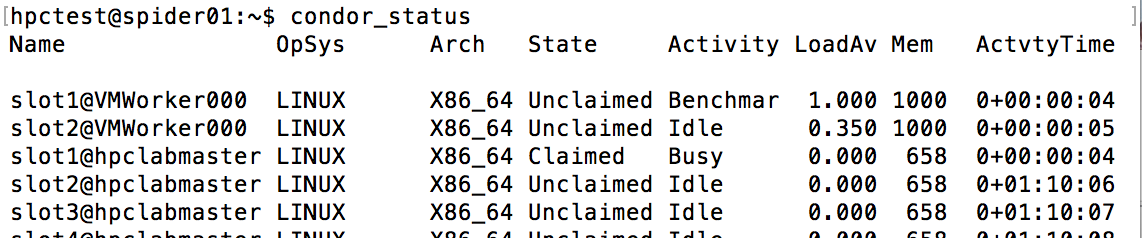
\includegraphics[width=0.9\textwidth]{Figures/vmwok.png}
\decoRule
\caption{Recursos de nuestra máquina en el pool}
\label{fig:condor creed}
\end{figure}
\FloatBarrier

\subsection{Configuración para Java}

Para poder usar el universo \textbf{Java}, no basta con tener el entorno de ejecución instalado, se debe descargar y configurar varios archivos, para que el nodo maestro \textbf{\textit{hpclabmaster}} pueda reconocer las máquinas que disponen de este entorno.

editamos el archivo: sources.list

\textbf{nano /etc/apt/sources.list}

y al final del mismo colocamos la linea siguiente:

\begin{figure}[h]
\centering

\includegraphics[width=1\textwidth]{Figures/sourceedit.png}
\decoRule
\caption{Repositorio fuente }
\label{fig:source}
\end{figure}
\FloatBarrier

Luego de esto descargamos la llave publica para HTCondor con el siguiente comando.

wget -qO - http://research.cs.wisc.edu/htcondor/debian/HTCondor-Release.gpg.key | sudo apt-key add -

Luego se descarga el archivo necesario para que htcondor reconozca y admita la máquina de trabajo como una que tiene el universo de Java disponible y habilitado. El archivo necesario para esto es : \textbf{\textit{scimark2lib.jar}}

nos movemos a la ruta: \textit{cd /usr/lib/condor/}

y allí ejecutamos el siguiente comando:

\textbf{wget http://math.nist.gov/scimark2/scimark2lib.jar}

Una vez descargado el archivo, se ejecutan los siguientes comandos, en orden para que condor reconozca los cambios realizados.

\textbf{apt update}

\textbf{apt dist-upgrade}

\textbf{apt install condor} (Este ultimo reinstala la herramienta para tomar los cambios realizados)

Reiniciamos el servicio HTCondor, y para confirmar que el universo java esta habilitado ejecutamos el comando :

\begin{lstlisting}
condor_status -java
\end{lstlisting} 
\begin{figure}[h]
\centering
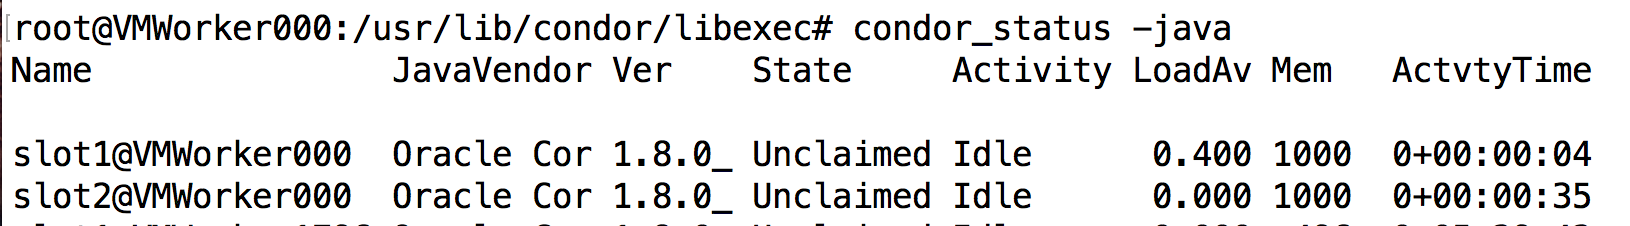
\includegraphics[width=1\textwidth]{Figures/javaready.png}
\decoRule
\caption{Universo Java Disponible }
\label{fig:Java Universe}
\end{figure}
\FloatBarrier

\textbf{NOTA:} Los pasos necesarios para el correcto funcionamiento del universo Java se realizan ya que en las nuevas distribuciones (versión 8.X en adelante) de la herramienta HTCondor no contienen el archivo de java necesario (\textbf{\textit{scimark2lib.jar}}) para que la herramienta reconozca las máquinas habilitadas con este universo.

Ahora la máquina esta lista para ser usada como nodo de trabajo en el cluster, en el apartado de pruebas se llevará a cabo una para mostrar la ejecución de trabajos en Java.


\section{Script adicional}

Como serán máquinas diferentes que tendrán los nodos de ejecución, es necesario diferenciarlas, para ello, se crea un script para bash para que cambie el nombre de la maquina en la primera ejecución de la misma, luego el script se elimina a si mismo evitando futuros cambios de nombre.

Para el nombre se usa el nombre seguido numero aleatorio , quedando de esta manera ejemplo \textit{VMWorker123456}

\begin{figure}[h]
\centering
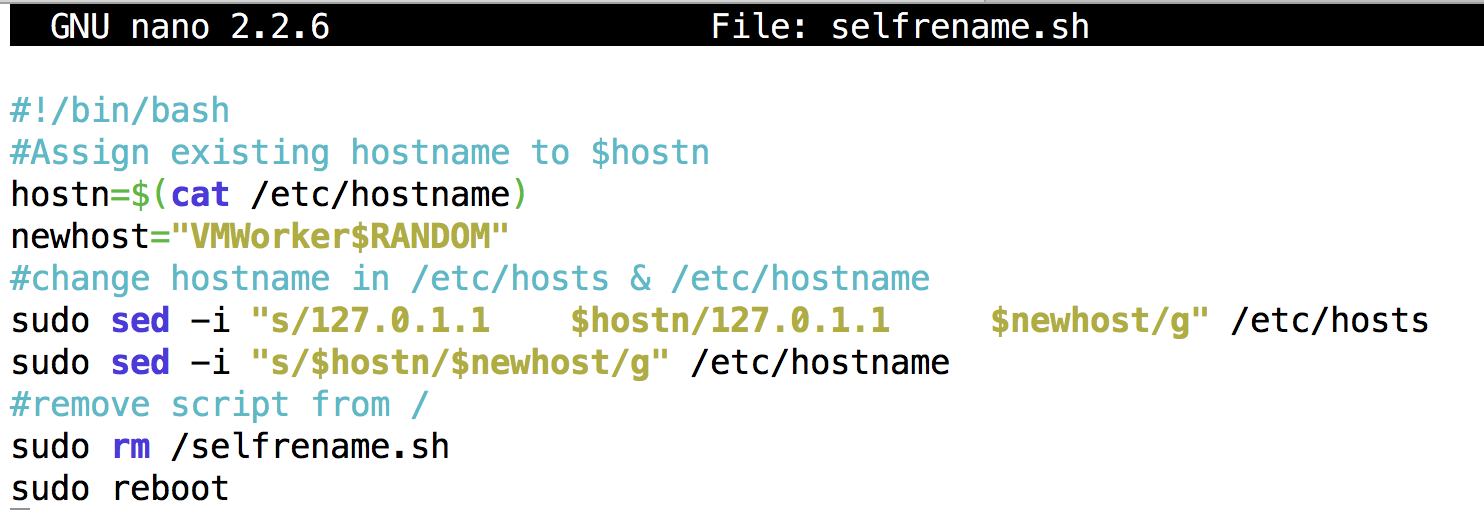
\includegraphics[width=1\textwidth]{Figures/scriptrename.png}
\decoRule
\caption{Script para renombrar la máquina }
\label{fig:rename script}
\end{figure}
\FloatBarrier

Este script modifica los archivos \textbf{\textit{hostname}} y \textbf{\textit{hosts}} que están en las rutas respectivas:

\textbf{\textit{/etc/hostname}} y \textbf{\textit{/etc/hosts}}

una vez creado el archivo, le damos permisos de ejecución con el comando:

\textbf{chmod a+x selfrename.sh}

luevo editamos el archivo \textit{rc.local} y agregamos el script para que se ejecute al iniciar la máquina.

\textbf{nano /etc/rc.local}

y al final colocamos la linea respectiva al script.

\begin{figure}[h]
\centering
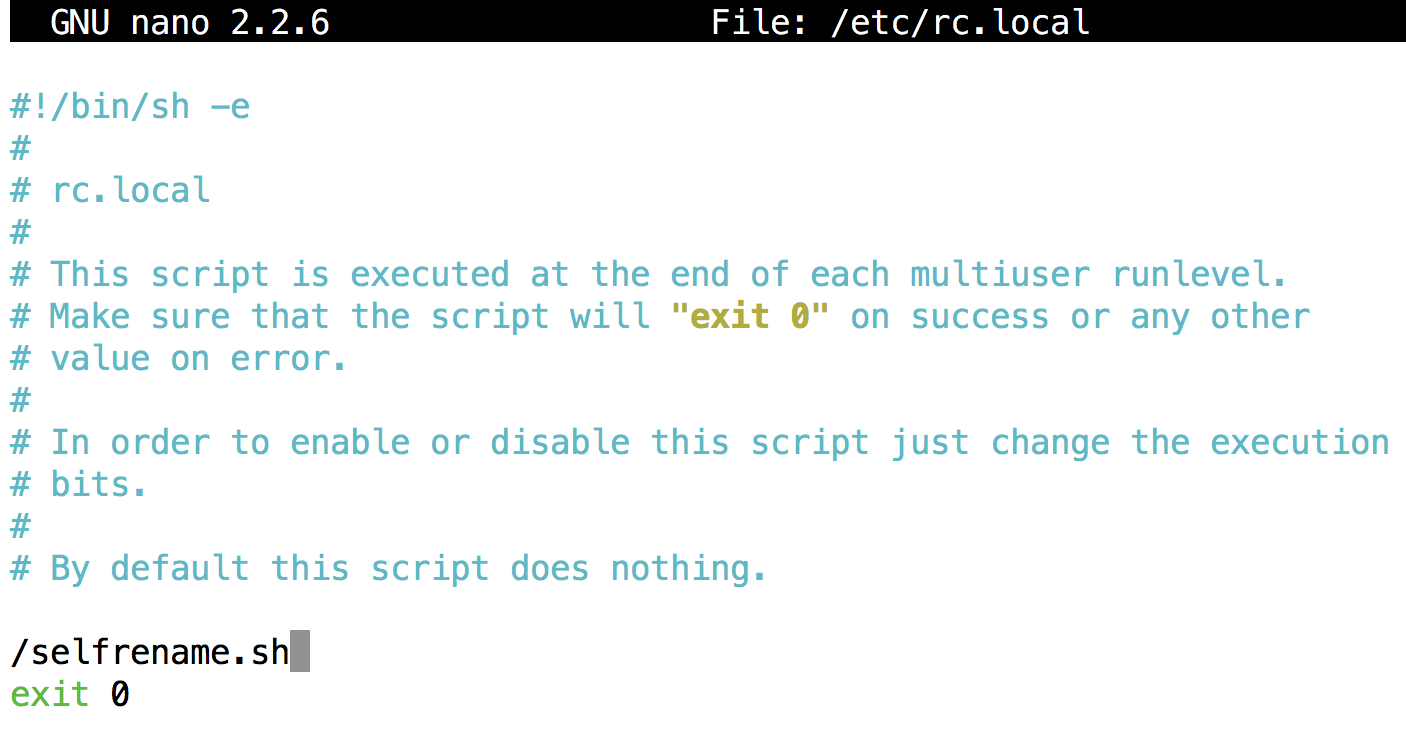
\includegraphics[width=1\textwidth]{Figures/rclocal.png}
\decoRule
\caption{Script para renombrar la máquina }
\label{fig:rename script}
\end{figure}
\FloatBarrier





%----------------------------------------------------------------------------------------- 
% Chapter Template

\chapter{Despliegue en Windows} % Main chapter title

\label{Chapter6} % Change X to a consecutive number; for referencing this chapter elsewhere, use \ref{ChapterX}

%----------------------------------------------------------------------------------------
%	SECTION 1
%-------------------------------------------------------------------------------
Para realizar el despliegue sobre las maquinas con sistema operativo Windows se necesitan dos herramientas básicas, adicional a el disco que contiene la imagen base de los nodos de trabajo.

Estas herramientas, son el gestos de máquinas virtuales \textbf{VirtualBox} y el aplicativo que ejecuta los nodos como servicios \textbf{VBoxVMService}.

Estas herramientas se pueden descargar de los enlaces en la Wiki del laboratorio de computación de alto desempeño de la Universidad Tecnológica de Bolívar o ingresando en el navegador la siguiente dirección dentro del campus:

\textit{http://172.16.9.80/ubuntu/spider/workers/}


\section{Pasos para el despliegue en Windows}

\subsection{Instalación de VirtualBox}
Es recomendado que se use la versión 5.0.18 de VirtualBox ya que es la actual al momento de realizar las pruebas. Pueden encontrar el instalador en el enlace de la Wiki.

Se des-instala cualquier versión anterior de VirtualBox y se realiza una instalación fresca de la versión 5.0.18, como administrador.

Una vez finalizada la instalación se procede a crear la máquina que sera el nodo de trabajo.

\subsection{Nodo de trabajo}

\subsubsection*{Creación máquina virtual}
Primero crearemos una máquina virtual con los parámetros de configuración óptimos de acuerdo a la máquina anfitrión (máquina Windows).

La creación de esta maquina es similar a la creación de la máquina base, ver el capitulo 4 de este mismo documento, el cambio esta al usar el Disco Virtual de la máquina base descargada del enlace de la wiki.

Movemos la imagen del disco virtual a la ruta: 

\begin{lstlisting}
C:\Users\"usuario"\VirtualBox VMs
\end{lstlisting}
Donde "usuario" sera remplazado por el nombre del usuario de la máquina windows, y descomprimimos allí nuestra imagen.

Luego al seleccionar la opción ‘‘usar disco virtual existente’’ y colocamos la ruta a nuestro disco virtual base y le damos ‘‘crea’’.

\begin{figure}[h]
\centering
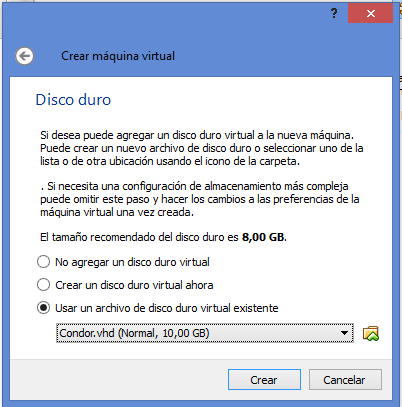
\includegraphics[width=0.8\textwidth]{windows/ddexistente.PNG}
\decoRule
\caption{Disco Virtual Base }
\label{fig:VHD Base}
\end{figure}
\FloatBarrier

Nuestra máquina es creada y procedemos a editar la configuración de esta.

\subsubsection*{Configuración máquina virtual}

Acedemos a la configuración mediante el icono del engranaje en VirtualBox.
Accedemos a la pestaña de sistema donde configuraremos la cantidad de memoria RAM a utilizar y el numero de procesadores.

Es recomendado utilizar el 25\%  de la cantidad total de RAM y el 50\% de los procesadores físicos (1 o 2 máximo).

\begin{figure}[h]
\centering
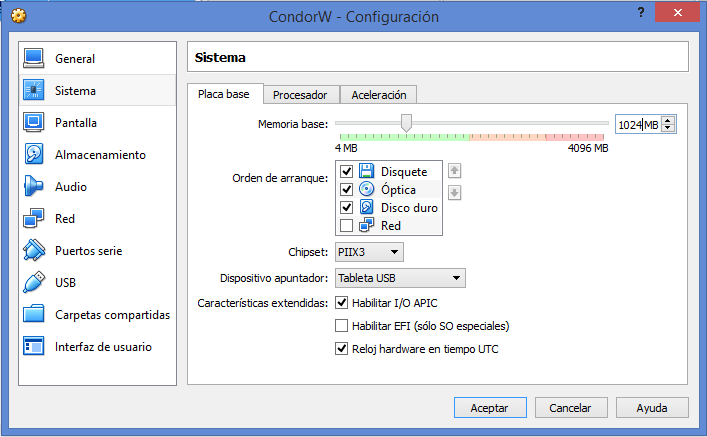
\includegraphics[width=0.8\textwidth]{windows/25ram.PNG}
\decoRule
\caption{Opciones de RAM y procesadores }
\label{fig:VM RAM}
\end{figure}
\FloatBarrier

Luego vamos a la pestaña de Red y colocamos el adaptador de red en modo puente (Bridge Mode), damos aceptar y la maquina esta lista para su primera ejecución.

\begin{figure}[h]
\centering
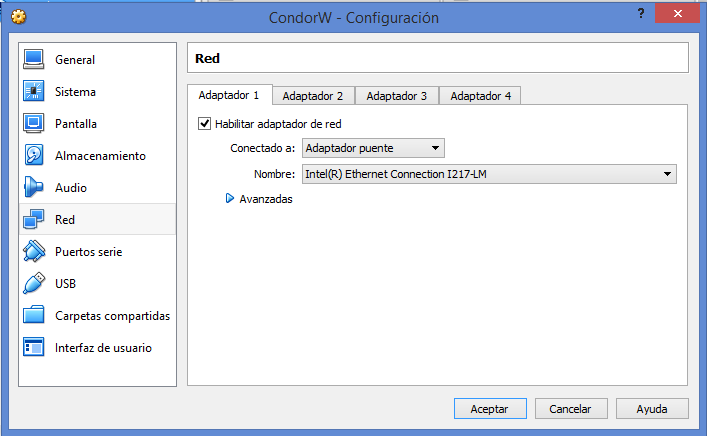
\includegraphics[width=0.8\textwidth]{windows/redpuente.PNG}
\decoRule
\caption{Red Adaptador Puente }
\label{fig:VM NET}
\end{figure}
\FloatBarrier

Ejecutamos la máquina y esperamos que termine la primera ejecución, puede ser algo demorado ya que se reinicia luego de cambiar su nombre.

\begin{figure}[h]
\centering
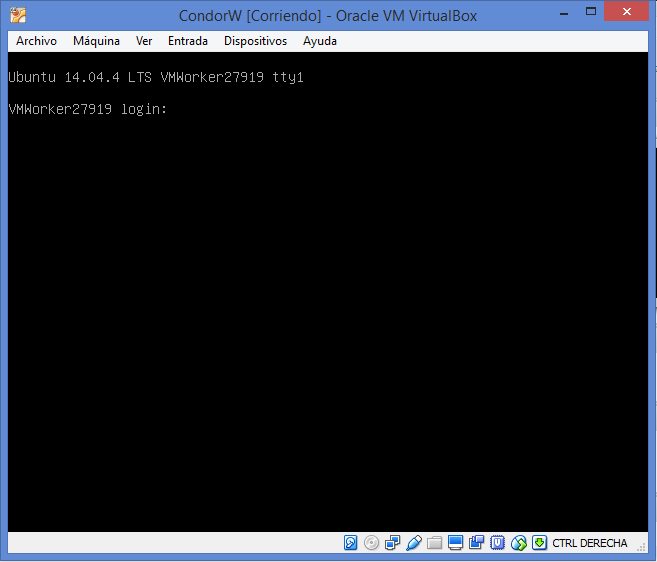
\includegraphics[width=0.9\textwidth]{windows/running.PNG}
\decoRule
\caption{Máquina virtual en funcionamiento}
\label{fig:VM Running}
\end{figure}
\FloatBarrier

Ahora se procede a configurar la máquina para ejecución en segundo plano, como servicio.

\subsubsection*{Máquina Virtual como servicio}

Para ejecutar la máquina virtual en background (no se creará ni se ejecutará la consola de administración de VirtualBox, ni la consola de ejecución de la máquina virtual) se instala la herramienta VBoxVMService.

Se cierra por completo VirtualBox y ejecutamos como administrador el instalador de VBoxVMService.
Se procede con la instalación sin cambiar la ubicación de instalación, una vez completada la instalación, finalizamos y vamos a la carpeta conde fue instalado.

\begin{lstlisting}
C:\vms
\end{lstlisting}

Allí se modifica el archivo \textbf{\textit{VBoxVmService}} que es el archivo de configuración.

\begin{figure}[h]
\centering
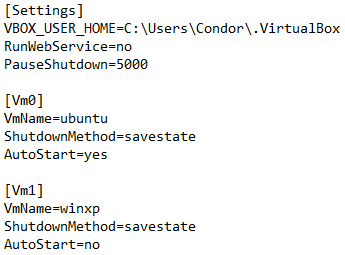
\includegraphics[width=0.75\textwidth]{windows/vmservice.PNG}
\decoRule
\caption{Archivo de configuración}
\label{fig:vms config}
\end{figure}
\FloatBarrier

Editamos los parámetros para que nuestra máquina virtual \textbf{\textit{CondorW}} inicie como servicio, y el método de apagado sea total, no guarde el estado en que se encontraba.

\begin{figure}[h]
\centering
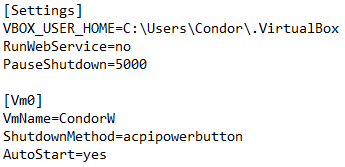
\includegraphics[width=0.75\textwidth]{windows/condorw.PNG}
\decoRule
\caption{Configuración final CondorW}
\label{fig:vms final}
\end{figure}
\FloatBarrier

Reiniciamos nuestra máquina anfitrión y nos aseguramos que al iniciar nuevamente nuestro nodo de trabajo se esta ejecutando en background.

\begin{figure}[h]
\centering
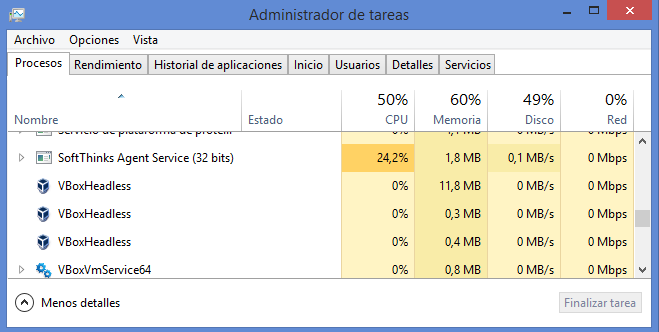
\includegraphics[width=0.75\textwidth]{windows/tasks.PNG}
\decoRule
\caption{Procesos en segundo plano en Windows}
\label{fig:task manager}
\end{figure}
\FloatBarrier

Se puede apreciar que esta en ejecución VBoxVmService y tres procesos Headless que son los que indican que nuestra maquina esta en ejecución en background.







%---------------------------------------------------------------------------
% Chapter Template

\chapter{Evidencias} % Main chapter title

\label{Chapter7} % Change X to a consecutive number; for referencing this chapter elsewhere, use \ref{ChapterX}

%----------------------------------------------------------------------------------------
%	SECTION 1
%----------------------------------------------------------------------------------------

\section{Pruebas de ejecución en universo Java}
Para hacer una prueba sencilla de ejecución en el universo Java, primero debemos crear un programa en java, compilarlo y luego enviarlo a la cola de trabajos de HTCondor. 

Para esta prueba usaremos un programa sencillo que hace un calculo y da una respuesta por terminal y luego veremos como se ejecuta este mismo trabajo en HTCondor.

\subsection{Creación y ejecución de la prueba}

primero creamos un archivo con nombre simple.java y lo editamos, y en el colocamos el contenido:
\begin{lstlisting}[frame=single,
  basicstyle=\footnotesize\ttfamily,
  language=Java, 
  numbers=left, 
  numberstyle=\tiny\color{black},
  captionpos=b]

\end{lstlisting}

\begin{figure}[h]
\centering
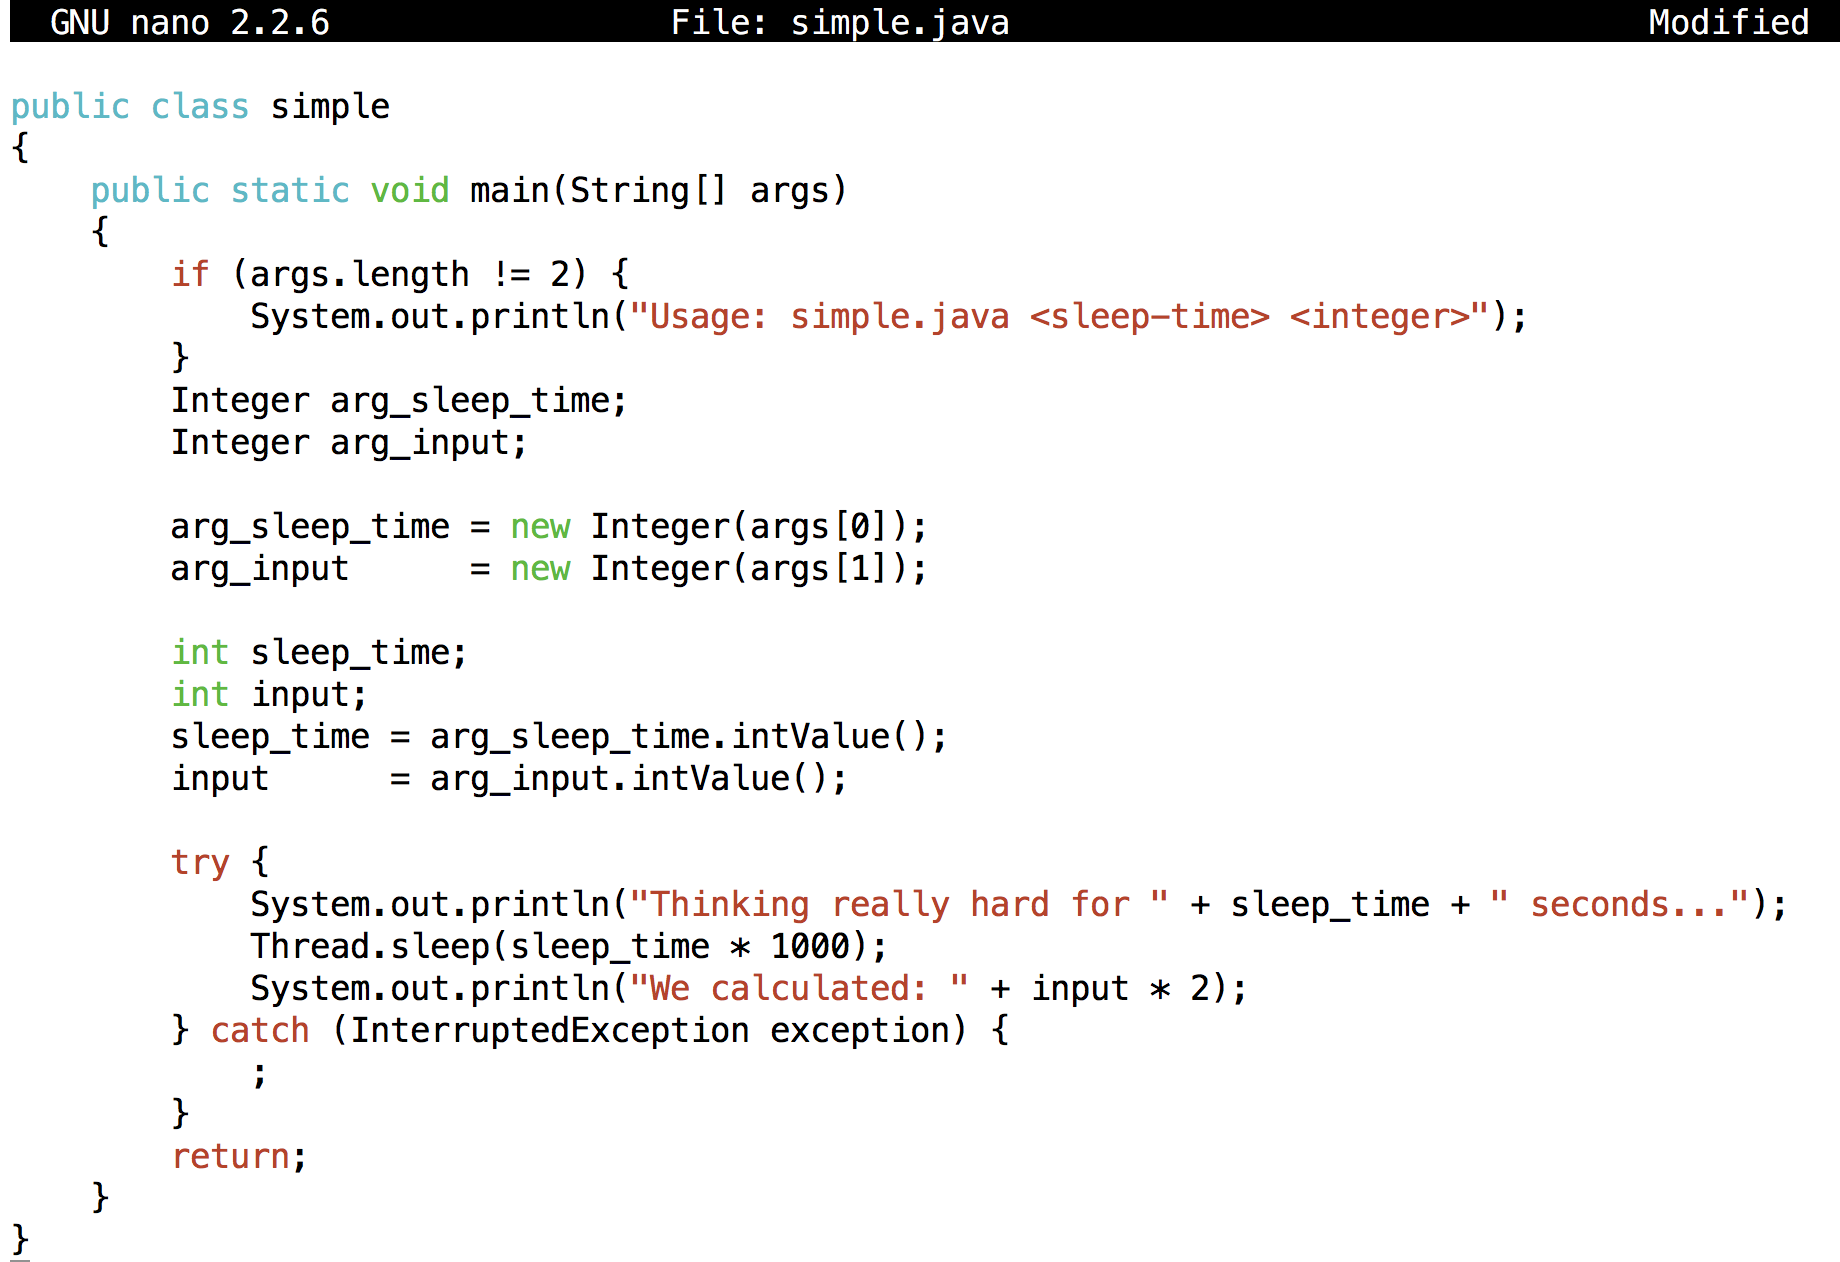
\includegraphics[width=0.9\textwidth]{images/simplejava.png}
\decoRule
\caption{Código prueba Java}
\label{fig:java test}
\end{figure}
\FloatBarrier


Luego compilamos el programa:

\textbf{javac simple.java}

Y lo ejecutamos:

\textbf{java simple 4 10}

nos arroja el resultado por terminal:

\begin{figure}[h]
\centering
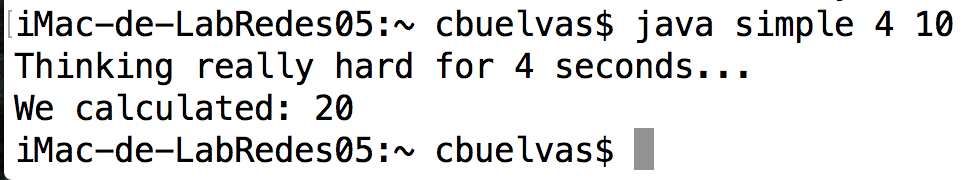
\includegraphics[width=0.8\textwidth]{images/resulttest.png}
\decoRule
\caption{Resultado ejecución local}
\label{fig:java test}
\end{figure}
\FloatBarrier

\subsection{Configuración de archivo ClassAd}

\subsubsection*{ClassAd}

HTCondor funciona mediante un mecanismo llamado \textbf{ClassAd},  este es un mecanismo flexible para la representación de las características y limitaciones de las máquinas y los trabajos (tareas) en HTCondor.
Dentro del sistema, los \textbf{ClassAd} pueden representar trabajos, recursos, nodos, máquinas remitentes y otros procesos de HTCondor.

Un ClassAd es un conjunto de expresiones de nombre exclusivo. Cada expresión nombrada se llama un atributo.

Enviamos a la maquina de envíos la prueba de java, y allí creamos el archivo de tarea que llamaremos \textbf{\textit{simple.job}}.

\textbf{Nota:} La extensión del archivo de tarea (submit file) puede ser cualquiera, luego que la configuración este realizada adecuadamente, utilizamos \textbf{.job} para mantener una idea clara de cual es su función.

El archivo de tarea quedara de la siguiente  manera.

\begin{lstlisting}[frame=single,
  basicstyle=\footnotesize\ttfamily,
  language=C, 
  numbers=left, 
  numberstyle=\tiny\color{black},
  captionpos=b]
Universe   = java
Executable = simple.class
Arguments  = simple 4 10
Log        = simple.log
Output     = simple.out.$(PROCESS)
Error      = simple.error
Rank       = (machine == "VMWorker24657")

should_transfer_files = YES
when_to_transfer_output = ON_EXIT

Queue 
\end{lstlisting}
  
Este archivo contiene toda la información necesaria para que HTCondor sepa donde ejecutar este trabajo. 

Los parámetros mostrados describen la configuración necesaria para la tarea.

\textbf{Universe}: Define el entorno de ejecución.

\textbf{Executable}: El archivo compilado que realizará la tarea 

\textbf{Arguments}: Los parámetros que recibe el archivo ejecutable.

\textbf{Log} : Crea un archivo con la información de la ejecución.

\textbf{Output}: Crea un archivo que contiene la salida de la ejecución.

\textbf{Error}: Crea un archivo de error con información en caso de fallas.

\textbf{Rank}: En esta prueba definimos que máquina del nodo queremos que ejecute la tarea.

\textbf{should\_transfer\_files} : define si se deben o no enviar archivos en el trabajo.

\textbf{when\_to\_transfer\_output}: especifica cuando transferir los resultados de la ejecución.

Para enviar el trabajo al cluster se usa el comando: \textit{\textbf{condor\_submit nombrearchivo.job}}

\begin{figure}[h]
\centering
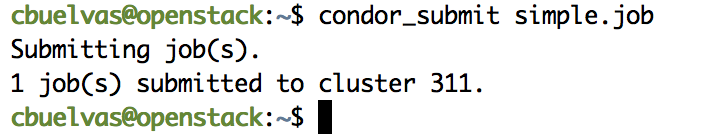
\includegraphics[width=0.8\textwidth]{images/submit.png}
\decoRule
\caption{Envío de trabajo al cluster}
\label{fig:condor submit}
\end{figure}
\FloatBarrier

Para verificar que el trabajo este en la cola se usa el comando : \textit{\textbf{condor\_q}}

\begin{figure}[h]
\centering
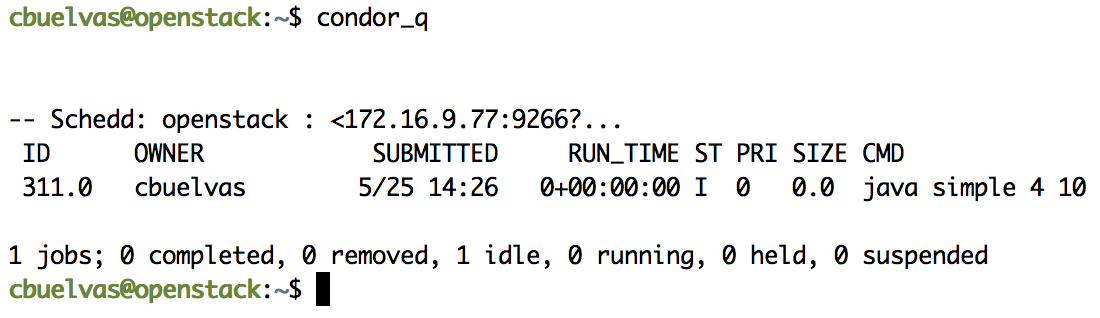
\includegraphics[width=1\textwidth]{images/condorq.png}
\decoRule
\caption{Cola de trabajo en el cluster}
\label{fig:condorq}
\end{figure}
\FloatBarrier

Verificación en el archivo simple.log del resultado de la ejecución.

\begin{figure}[h]
\centering
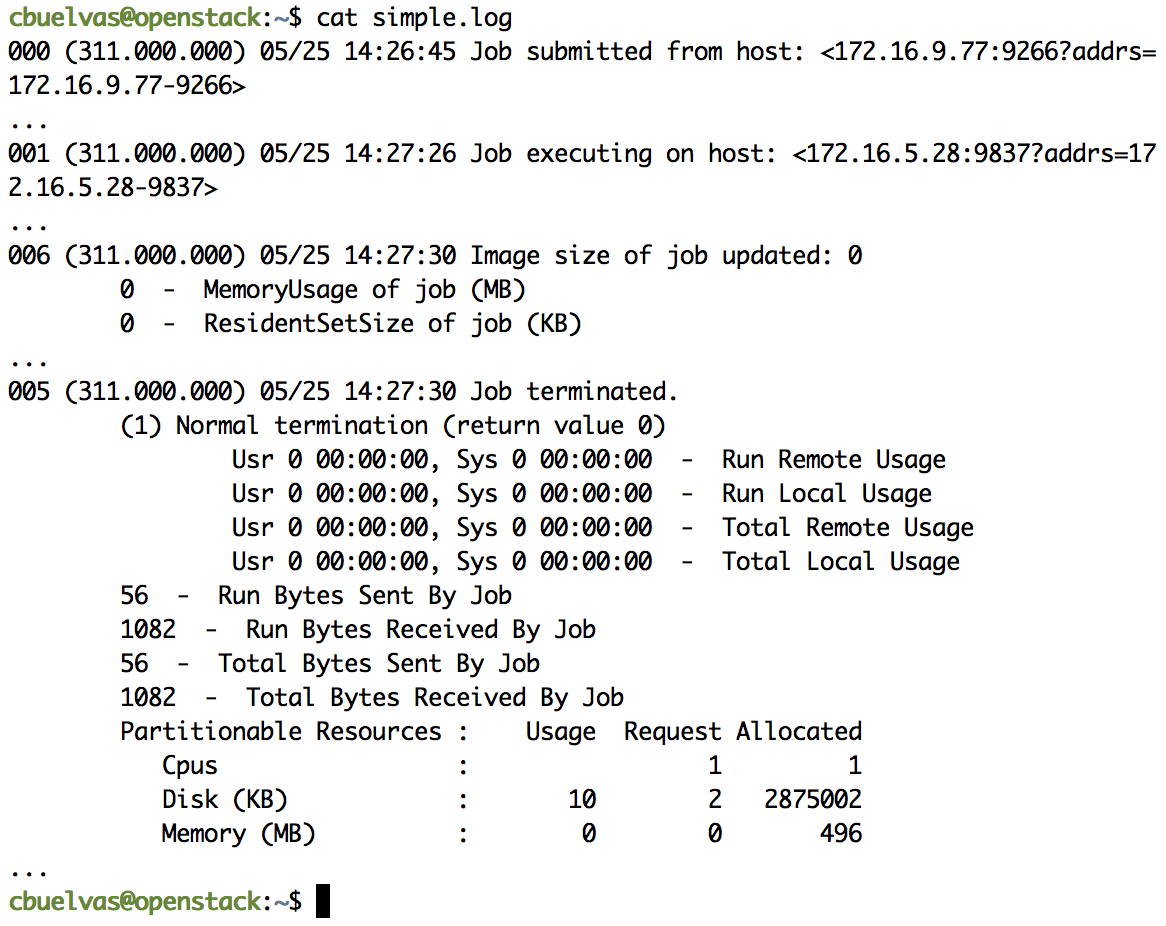
\includegraphics[width=0.9\textwidth]{images/sublog.png}
\decoRule
\caption{Log de envío}
\label{fig:file log}
\end{figure}
\FloatBarrier

Por ultimo verificamos el archivo de salida, que contiene los resultados de la ejecución.

\begin{figure}[h]
\centering
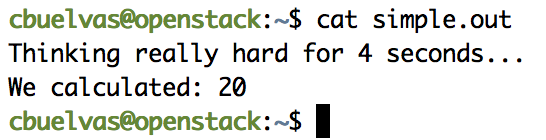
\includegraphics[width=0.8\textwidth]{images/simpleout.png}
\decoRule
\caption{Resultado prueba Java}
\label{fig:file log}
\end{figure}
\FloatBarrier

\section{Prueba de ejecución con Python}

Para esta prueba de ejecución, se calculara el tiempo de respuesta que le lleva a una maquina retornar el calculo y suma de los números primos en un rango dado. La prueba se ejecuta primero haciendo uso de multithreads y luego en serial, y arrojara el resultado en un archivos el cual se puede examinar una vez completado el trabajo.

\subsubsection*{Prueba en local}

El script que ejecutara el calculo es el siguiente:

\begin{lstlisting}[basicstyle=\footnotesize\ttfamily,
  language=Python, 
  numbers=left, 
  numberstyle=\tiny\color{black},
  captionpos=b]
#!/usr/bin/python
import multiprocessing as mp
from Queue import Empty
import math
import os
import time
def primeQ(n):
    """return a boolean, is the input integer a prime?"""
    if n == 2 :
        return True
    max =  int( math.ceil( math.sqrt(n) ) )
    i = 2
    while i <= max :
        if n % i == 0 :
            return False
        i += 1
    return True

def sumPrimes(n):
    """return sum of all primes less than n """
    return sum( [ x for x in range(2,n) if primeQ(x) ] )

def worker(q):
    while True:
        try:
            x = q.get(block=False)
            print sumPrimes(x)
        except Empty:
            break
if __name__ == "__main__":
    start = time.time()
ncpus = 4
my_q  = mp.Queue()
for i in range(100000, 2000000, 100000):
    my_q.put(i)
procs=[mp.Process(target=worker, args=(my_q,))  for i in range(ncpus)]
for ps in procs:
    ps.start()
for ps in procs:
    ps.join()
mid  = time.time()
print "now the serial part "
for i in range(100000, 2000000, 100000):
    print sumPrimes(i)
ending = time.time()
print "multiprocessing takes ", mid - start,      " seconds"
print "single thread takes ",      ending - mid,  " seconds"
\end{lstlisting}

Luego de creado el y editado el archivo se guarda el archivo como \textbf{primes} y se le da permisos de ejecución con el comando : \textbf{chmod a+x primes}.

Lo ejecutamos de manera local y vemos el resultado en la terminal:

\begin{figure}[h]
\centering
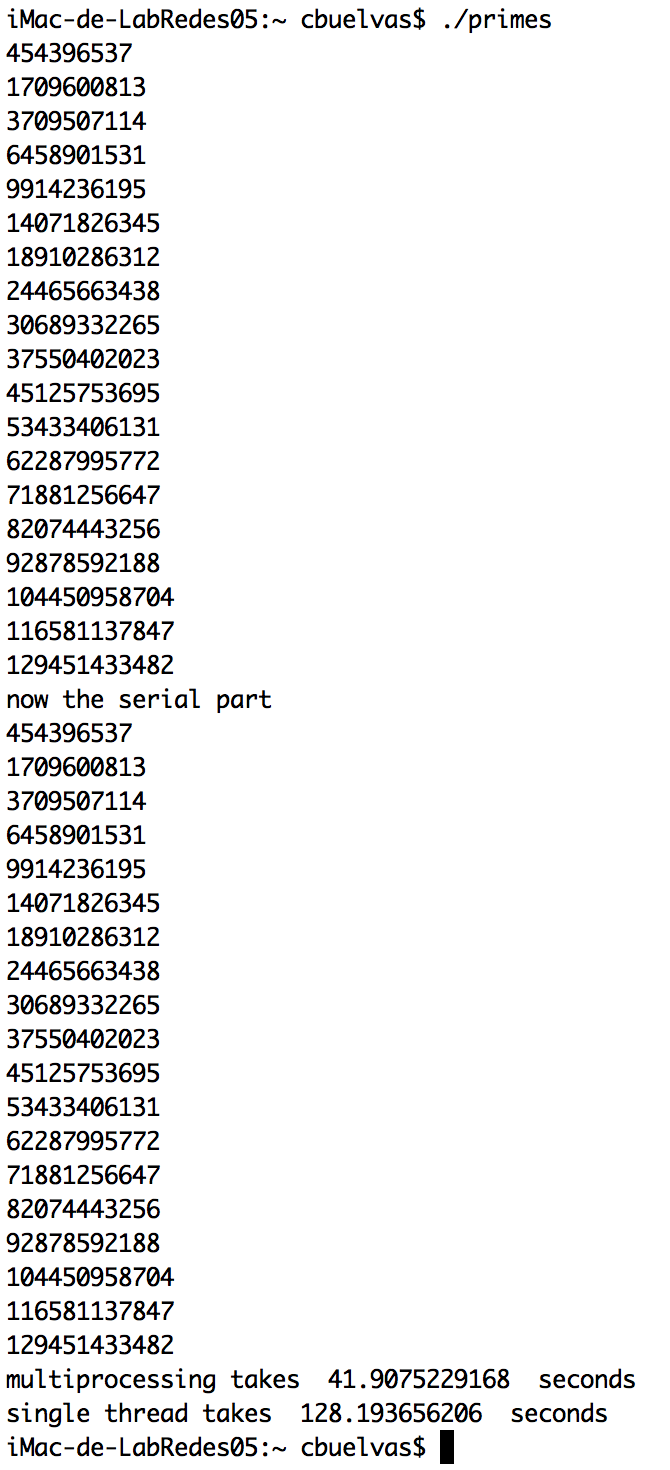
\includegraphics[width=0.8\textwidth]{images/localpython.png}
\decoRule
\caption{Ejecución de la prueba local}
\label{fig:python local test}
\end{figure}
\FloatBarrier

Luego llevamos este script a una máquina de envíos de trabajo y editamos el archivo ClassAd de envío y el script con la tarea.

Nuestro script es el mismo, se muestra como se configura el script para enviar las tarea:

\begin{figure}[h]
\centering
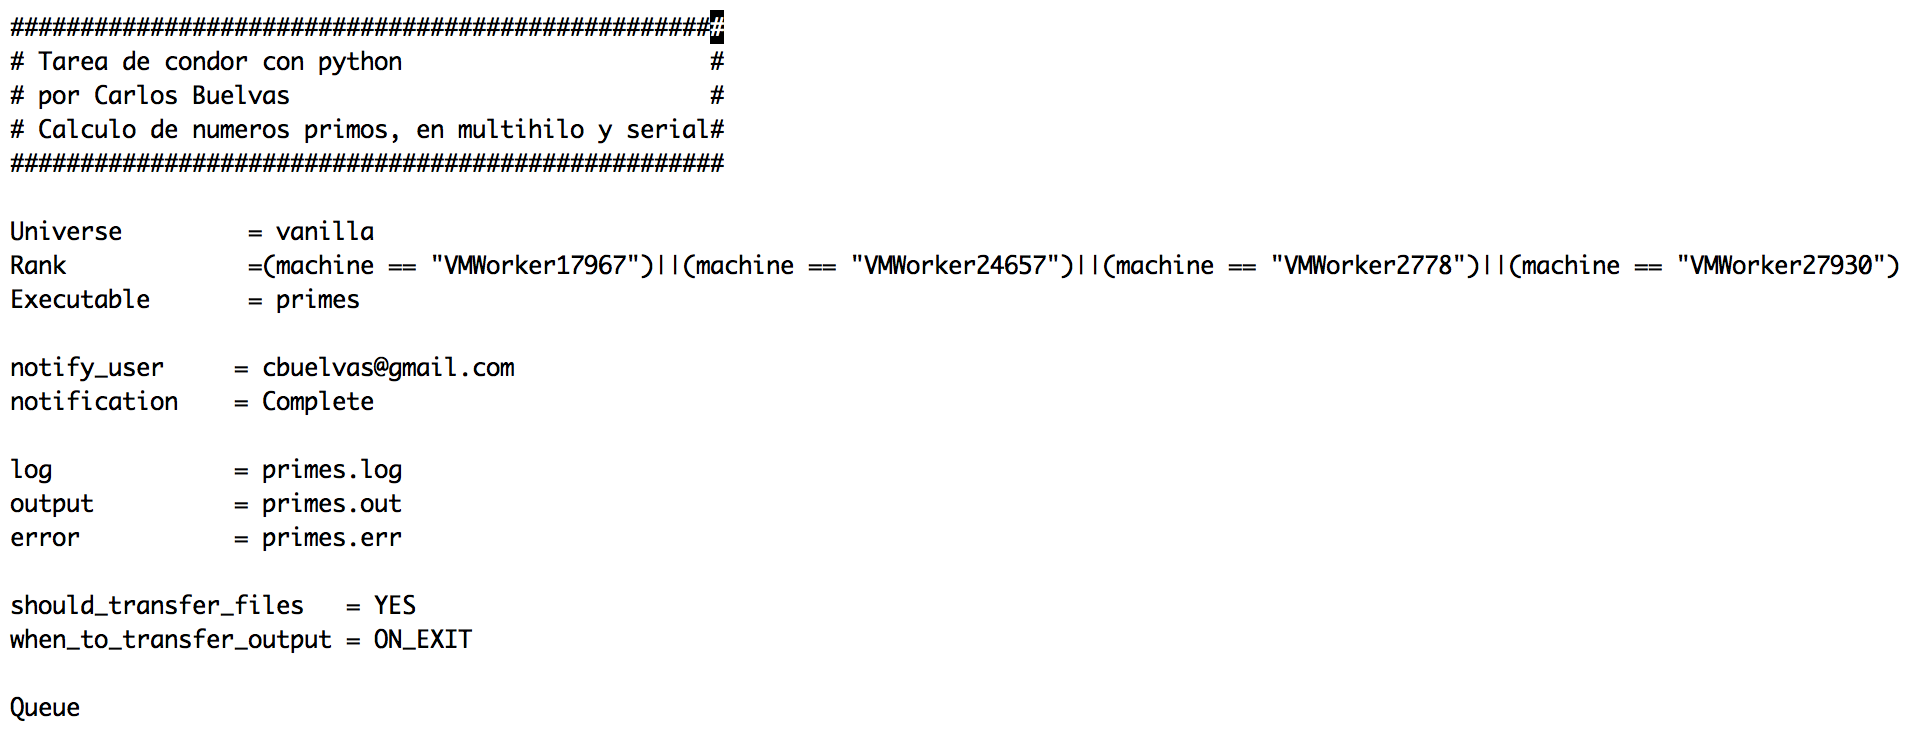
\includegraphics[width=1\textwidth]{images/pythonsub.png}
\decoRule
\caption{ClassAd para el envío al cluster}
\label{fig:python submit}
\end{figure}
\FloatBarrier

Enviamos el trabajo al cluster y verificamos que este en cola de trabajo.

\begin{figure}[h]
\centering
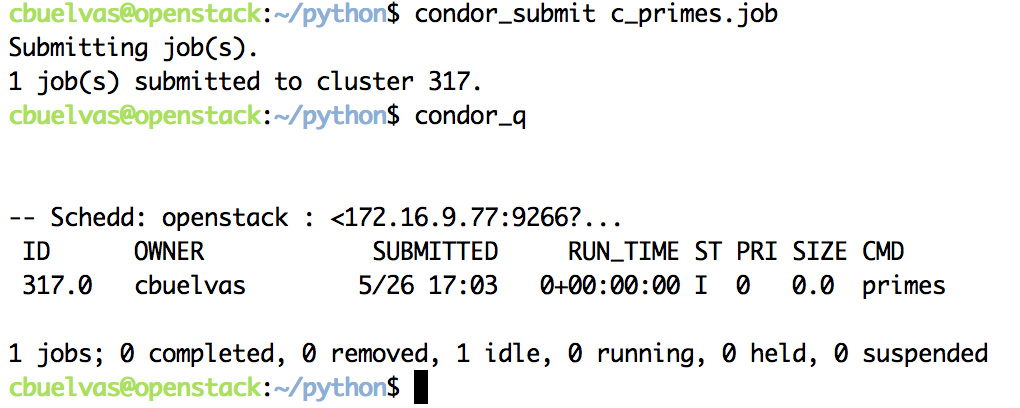
\includegraphics[width=0.8\textwidth]{images/condorsub.png}
\decoRule
\caption{Envío del trabajo y verificación de la cola de trabajos}
\label{fig:condor submit and q}
\end{figure}
\FloatBarrier

Luego podemos ver la información de la ejecución en el archivo de \textbf{\textit{log}}.
\begin{figure}[h]
\centering
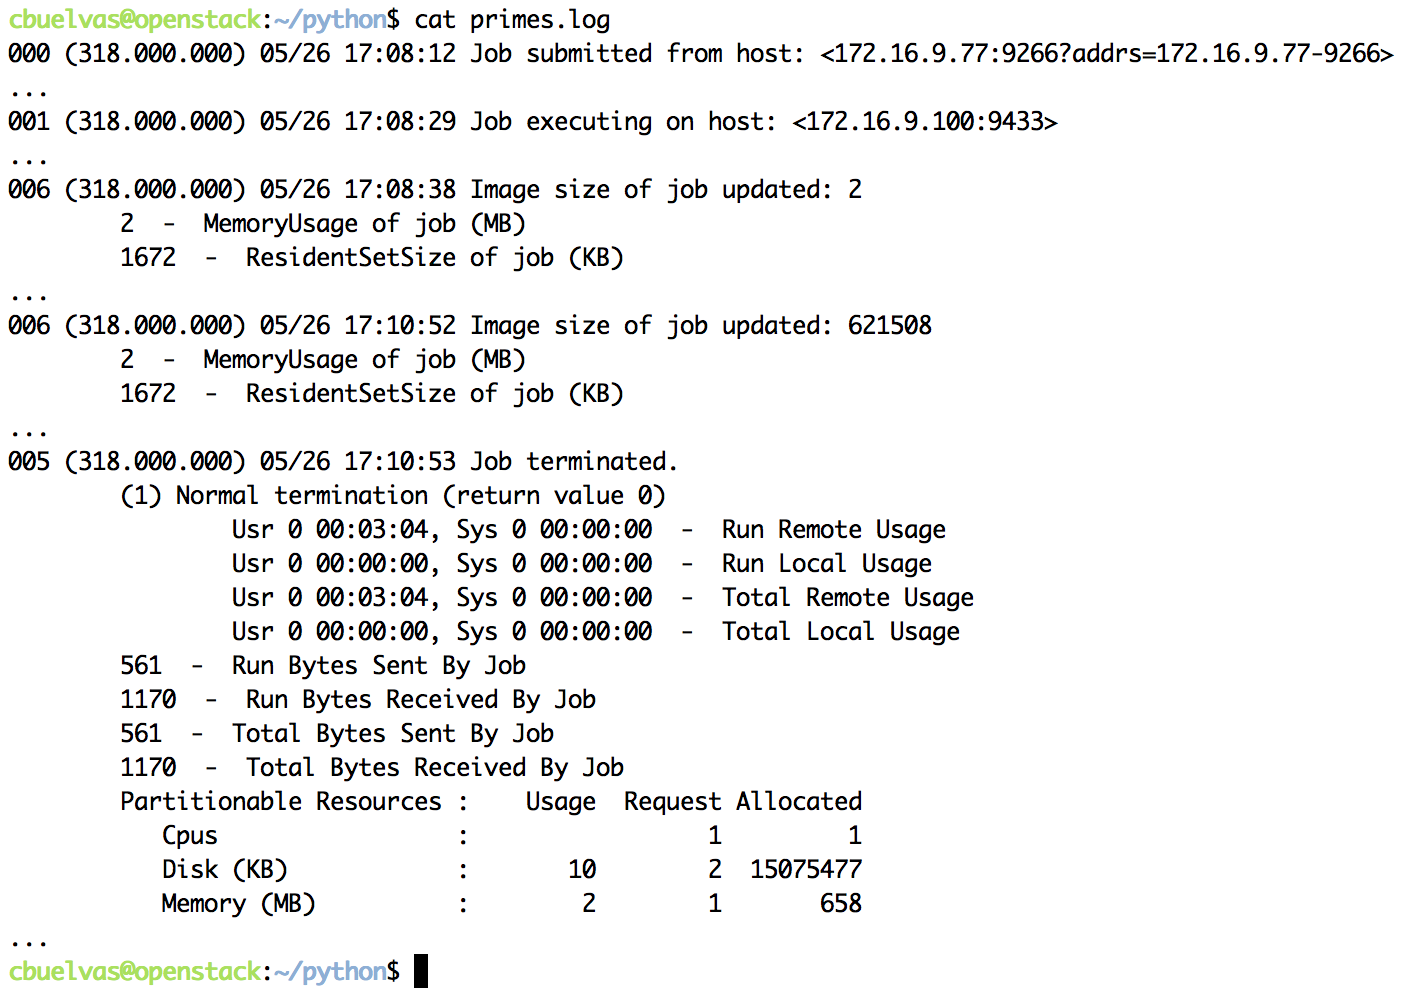
\includegraphics[width=1\textwidth]{images/pythonlog.png}
\decoRule
\caption{Log de ejecución de la prueba}
\label{fig:python log}
\end{figure}
\FloatBarrier
 Y el resultado de la ejecución lo vemos en el archivo de salida \textbf{\textit{.out}}.
 
 \begin{figure}[h]
\centering
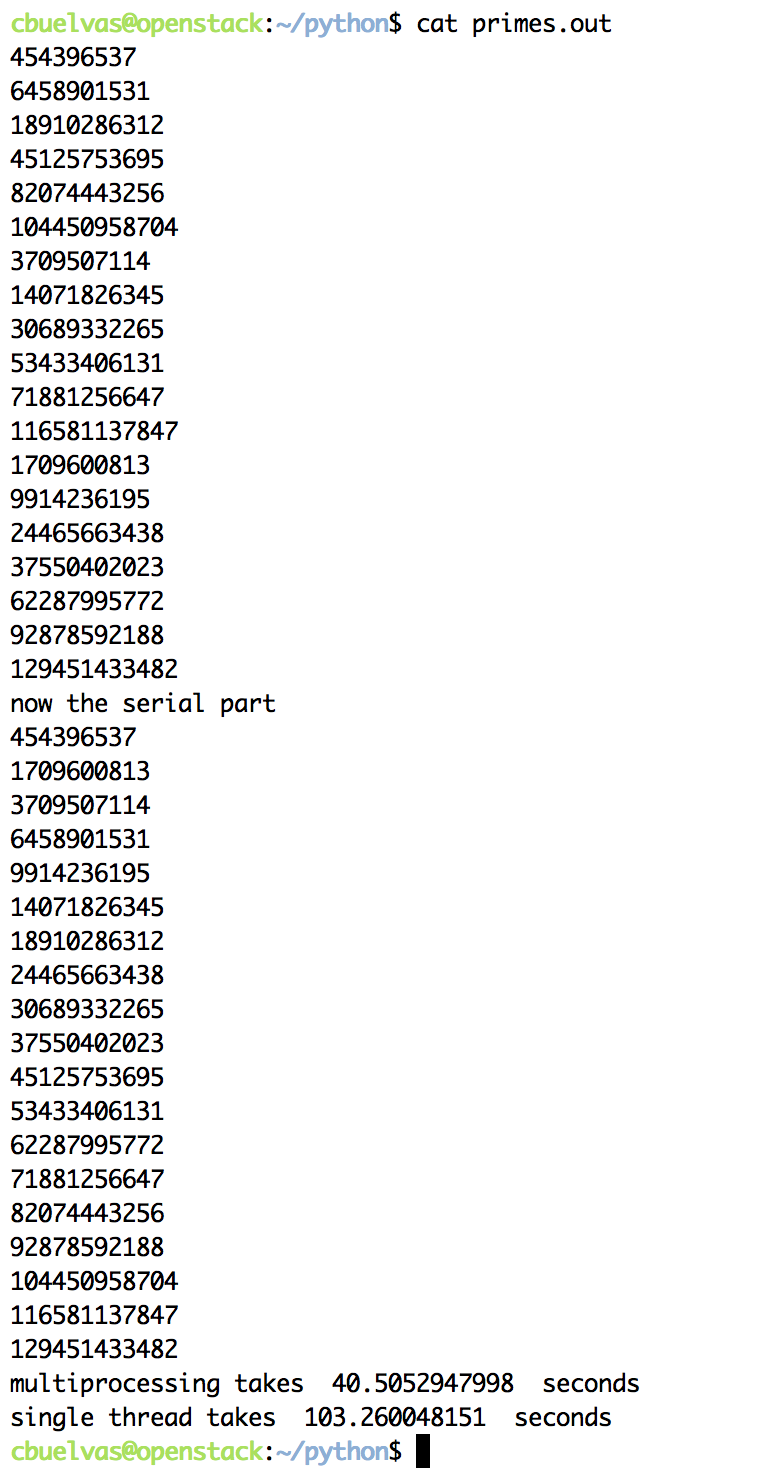
\includegraphics[width=0.8\textwidth]{images/clusterout.png}
\decoRule
\caption{Resultado de la ejecución}
\label{fig:python out}
\end{figure}
\FloatBarrier

con esto vemos que los entornos de ejecución para los cuales se diseño esta solución, están activos y son funcionales.

\section{Trabajos Futuros}

Al desarrollar este trabajo, se encontraron diferentes obstáculos a la hora de usar la herramienta HTCondor, entre ellas hay configuraciones de seguridad que se deben tener en cuenta.
\begin{itemize}
	\item Para lograr correcta comunicación entre los nodos de ejecución y el nodo maestro, todos deben pertenecer al mismo dominio (Ej, dominio.local.edu), para ello se deben configurar a la hora de instalar los equipos este dominio.
    \item Para aumentar la cantidad de nodos de trabajo, este trabajo se debe replicar en todos los salones de computo del campus.
    \item El nodo maestro, actualmente por pruebas esta aceptando los trabajos de cualquier dominio, esta es una falla de seguridad.
    \item Para hacer parte, y hacer uso de clusters de otras universidades, se debe configurar Flokking entre clusters.
\end{itemize}






%-----------------------------------------------
%----------------------------------------------------------------------------------------
%	THESIS CONTENT - APPENDICES
%----------------------------------------------------------------------------------------

\appendix % Cue to tell LaTeX that the following "chapters" are Appendices

% Include the appendices of the thesis as separate files from the Appendices folder
% Uncomment the lines as you write the Appendices

%% Appendix A

\chapter{Appendix Title Here} % Main appendix title

\label{AppendixA} % For referencing this appendix elsewhere, use \ref{AppendixA}

Write your Appendix content here.
%\include{Appendices/AppendixB}
%\include{Appendices/AppendixC}

%----------------------------------------------------------------------------------------
%	BIBLIOGRAPHY
%----------------------------------------------------------------------------------------

\printbibliography[heading=bibintoc]
%\bibliography{referencias.bib}
%----------------------------------------------------------------------------------------

\end{document}  
